% !TEX root=/home/tavant/these/manuscript/src/manuscript.tex

\documentclass[
   a4paper,	%Pour papier A4
   12pt,		%Taille de la police 12
   twoside,	%recto-verso
   headinclude, headsepline, plainheadsepline,
   bibliography=totoc, toc=listof,
   numbers=noenddot,
   captions=tableheading,
   % fleqn,   % left alignment of formula
   amsmath, hidelinks  ]{book}
   %Packages
% !TEX root=/home/tavant/these/manuscript/src/manuscript.tex

\usepackage[english,french]{babel}


% -------------
% font spec
%-----------
\usepackage[T1]{fontenc}
% \usepackage{ebgaramond}

\usepackage{titlesec}
\usepackage{titling}
% Specify different font for section headings
\newcommand*{\headingfont}{\fontfamily{phv}\selectfont}

\titleformat*{\section}{\LARGE\headingfont}
\titleformat*{\subsection}{\Large\headingfont}
\titleformat*{\subsubsection}{\large\headingfont}

%use \showfont to print the current font used
\makeatletter
\newcommand{\showfont}{encoding: \f@encoding{},
  family: \f@family{},
  series: \f@series{},
  shape: \f@shape{},
  size: \f@size{}
}
\newcommand{\iffont}[3]{\ifthenelse{\equal{\f@family}{#1}}{#2}{#3}}
\makeatother



\usepackage{lmodern}% http://ctan.org/pkg/lm for allowing arbitrary font size
\newcommand{\hsc}[1]{{\footnotesize\MakeUppercase{#1}}}   % Fake Small Caps

\usepackage[latin1]{inputenc}
\usepackage{eso-pic}	%eso-pic pour mettre des images avant les chapitres
\usepackage{float, caption}
\usepackage{amsmath,amssymb,mathrsfs,amsfonts}
\usepackage[amssymb]{SIunits}

\usepackage[thmmarks,amsmath]{ntheorem}
\usepackage{array, multirow, tabularx}
\usepackage{mathrsfs}                   %pour faire des cursives dans les formules

\usepackage{SIunits}		        %SI units
\usepackage{listings}		        %Pour ecrire du code
\usepackage[final]{pdfpages}		%Pour insérer des feuilles pdf (page de garde+abstracts)
\usepackage{minitoc} 			%Pour faire des mini tables des matières en début de chapitre

\usepackage{xcolor} %pour avoir les couleurs



\usepackage[nocfg]{nomencl}
\renewcommand{\nomname}{List of Symbols}
\makenomenclature

\usepackage{textcomp} %pour les apostrophes
\usepackage[nottoc,numbib,notlof,notlot]{tocbibind} %pour afficher l'entrée biblio dans la table des matières
%\usepackage[firstpage]{draftwatermark} %pour marquer draft sur la première page
%\SetWatermarkScale{6} %taille de la watermark
%\SetWatermarkLightness{0.9} %transparence de la watermark


% GRAPHICS
\usepackage{graphicx}
\usepackage{subfig}	%pour mettre des subplots
\graphicspath{{images/}{Chapitre1/}{Chapitre1/figure/}{schemas/}{plots/}{images/}{logos/}}  % Location of the graphics files (set up for graphics to be in PDF format)


\usepackage{etoolbox}
\patchcmd{\chapter}{plain}{empty}{}{}


\definecolor{lightgray}{gray}{0.95}
\hyphenation{Fortran}		        %Pour eviter l'hyphenation de "Fortran"

\lstset{language=[90]Fortran,	%Pour bien ecrire le code en Fortran
  basicstyle=\fontsize{11}{13}\selectfont\ttfamily,
  keywordstyle=\color{gray},
  commentstyle=\color{blue},
  morecomment=[l]{!\ },  %Comment only with space after !
  captionpos=b, % sets the caption-position to bottom
  frame=single, % adds a frame around the code
  %numbers=left, % where to put the line-numbers
  %numbersep=5pt, % how far the line-numbers are from the code
  %stepnumber=2, % the step between two line-numbers
  rulecolor=\color{black}, % if not set, the frame-color may be changed
  backgroundcolor=\color{lightgray}, % choose the background color
  breaklines=true %break lines if too long
}

% TODO: Fix Greek mu

\usepackage[activate={true,nocompatibility},final,tracking=true,kerning=true,spacing=true,factor=1100,stretch=10,shrink=10]{microtype}
% activate={true,nocompatibility} - activate protrusion and expansion
% final - enable microtype; use "draft" to disable
% tracking=true, kerning=true, spacing=true - activate these techniques
% factor=1100 - add 10% to the protrusion amount (default is 1000)
% stretch=10, shrink=10 - reduce stretchability/shrinkability (default is 20/20)


% For better intext references. By example \cref{fig:X} produces "Fig. n° X" instead of just "X"
\usepackage{varioref} % add the page when the object is far away

\ifpdf
  \usepackage[pagebackref=true,hyperindex=true,colorlinks=true]{hyperref}
  \hypersetup{pdfstartview={FitH}, bookmarksnumbered={true}}

\else
  \usepackage[hypertex=true,hyperindex=true,colorlinks=false]{hyperref}
\fi
\hypersetup{
    colorlinks,
    linkcolor={red!50!black},
    citecolor={blue!50!black},
    urlcolor={blue!80!black}
}

\usepackage[capitalise]{cleveref}  %hance, uyse \vref for the page reference, else \cref only


% For better citations.
\usepackage[numbers]{natbib}
%\usepackage[style=phys]{biblatex}

%~~~~~~~~~~~~~~~~~~~~~~~~~~~~~~
%  Overlay bar for means
\makeatletter
\newsavebox\myboxA
\newsavebox\myboxB
\newlength\mylenA
\usepackage[super]{nth}

\newcommand*\mean[2][0.75]{%
    \sbox{\myboxA}{$\m@th#2$}%
    \setbox\myboxB\null% Phantom box
    \ht\myboxB=\ht\myboxA%
    \dp\myboxB=\dp\myboxA%
    \wd\myboxB=#1\wd\myboxA% Scale phantom
    \sbox\myboxB{$\m@th\overline{\copy\myboxB}$}%  Overlined phantom
    \setlength\mylenA{\the\wd\myboxA}%   calc width diff
    \addtolength\mylenA{-\the\wd\myboxB}%
    \ifdim\wd\myboxB<\wd\myboxA%
       \rlap{\hskip 0.5\mylenA\usebox\myboxB}{\usebox\myboxA}%
    \else
        \hskip -0.5\mylenA\rlap{\usebox\myboxA}{\hskip 0.5\mylenA\usebox\myboxB}%
    \fi}
\makeatother


% !TEX root=/home/tavant/these/manuscript/src/manuscript.tex



\usepackage{xargs}                      % Use more than one optional parameter in a new commands
% \usepackage[pdftex,dvipsnames]{xcolor}  % Coloured text etc.
\usepackage[colorinlistoftodos,prependcaption,textsize=small]{todonotes}

\newcommandx{\unsure}[2][1=]{\todo[inline,linecolor=red,backgroundcolor=red!25,bordercolor=red,#1]{#2}}

\newcommandx{\change}[2][1=]{\todo[inline,linecolor=blue,backgroundcolor=blue!25,bordercolor=blue,#1]{#2}}

\newcommandx{\info}[2][1=]{\todo[inline,linecolor=OliveGreen,backgroundcolor=OliveGreen!25,bordercolor=OliveGreen,#1]{#2}}

\newcommandx{\improvement}[2][1=]{\todo[inline,linecolor=red,backgroundcolor=red!25,bordercolor=red,#1]{#2}}

\newcommandx{\thiswillnotshow}[2][1=]{\todo[noline,disable,#1]{#2}}
\newcommandx{\inlinenote}[2][1=]{\todo[inline,size=\small,#1]{#2}}



\usepackage{acronym}  %to handle acronym


% Define the abstract Env.
\usepackage{fancyhdr}
\pagestyle{empty}

\newenvironment{abstract}%
    {\cleardoublepage\thispagestyle{empty}\null\vfill\begin{center}%
    \bfseries\abstractname\end{center}}%
    {\vfill\null}


% ignore bibliorapgy if empty
\let\myBib\thebibliography

\renewcommand\thebibliography[1]{\ifx\relax#1\relax\else\myBib{#1}\fi}

%for linebreak
\renewcommand\linebreak{\vspace{1em}}



\newenvironment{zzz}
               {\list{}{\rightmargin0pt \leftmargin4em }%
                \item\relax}
               {\endlist}

\newcommand\subfigurewidth{2in}
\newcommand\defaultwidth{4in}

\usepackage[]{algorithm2e}
 \usepackage{mathtools}


 %===================
 % Subfigures
\usepackage[percent]{overpic}

\newcommand\subfiguretics[3]{
\begin{overpic}[width=\subfigurewidth,grid,tics=10]{#1}
 \put (#3) {\bf #2}
\end{overpic}
}
\newcommand\subfigure[3]{
\begin{overpic}[width=\subfigurewidth]{#1}
 \put (#3) {\bf #2}
\end{overpic}
}


\pdfcompresslevel=0

\selectlanguage{english}%

% ===============================
%   INCLUDE
% ===============================
\includeonly{structure/structure,%
 structure/lists,%
 Context/0_concepts,%
 Chapitre1/1-introduction,%
 % Chapitre2/2-mean_values,%
 % Chapitre3/3-non_isothermal_sheath,%
 % Chapitre4/4-polytropic_SEE,%
 % Chapitre5/5-ECDI, %
 texfiles/1ere
 }

 
% !TEX root=/home/tavant/these/manuscript/src/manuscript.tex

%%%%%%%%%%%%%%%%%%%%%%%%%%%%%%%%%%%%%%%%%%%%%%%%%%%%%%%%%%%%%%%%%%%%%%%%%%%%%%%%%%%%%%%%%%%%%%%%%%%%%%%%%%%%%%%%%%%%%%%%%%%%%%%%%%%%%%%%%%%%%%%%%%%%%%%%%%%%%%%%%%%%%%%
%%%%%%%%%%%%%%%%%%%%%%%%%%%%%%%%%%%%%%%%%%%%%%%%%%%%%%%%%%%%%%%%%%%%%%%%%%%%%%%%%%%%%%%%%%%%%%%%%%%%%%%%%%%%%%%%%%%%%%%%%%%%%%%%%%%%%%%%%%%%%%%%%%%%%%%%%%%%%%%%%%%%%%%
%%% Modèle pour la 1ère de couverture des thèses préparées à l'Université Paris-Saclay, basé sur le modèle produit par Guillaume BRIGOT / Template for back cover of thesis made at Université Paris-Saclay, based on the template made by Guillaume BRIGOT
%%% Mis à jour par Aurélien ARNOUX (École polytechnique)/ Updated by Aurélien ARNOUX (École polytechnique)
%%% Les instructions concernant chaque donnée à remplir sont données en bloc de commentaire / Rules to fill this file are given in comment blocks
%%% ATTENTION Ces informations doivent tenir sur une seule page une fois compilées / WARNING These informations must contain in no more than one page once compiled
%%%%%%%%%%%%%%%%%%%%%%%%%%%%%%%%%%%%%%%%%%%%%%%%%%%%%%%%%%%%%%%%%%%%%%%%%%%%%%%%%%%%%%%%%%%%%%%%%%%%%%%%%%%%%%%%%%%%%%%%%%%%%%%%%%%%%%%%%%%%%%%%%%%%%%%%%%%%%%%%%%%%%%%
%%% Version du 19 juillet 2018 (Merci à Hadrien VROYLANDT (Univ. Paris-Sud) pour ses suggestions et corrections)
%%%%%%%%%%%%%%%%%%%%%%%%%%%%%%%%%%%%%%%%%%%%%%%%%%%%%%%%%%%%%%%%%%%%%%%%%%%%%%%%%%%%%%%%%%%%%%%%%%%%%%%%%%%%%%%%%%%%%%%%%%%%%%%%%%%%%%%%%%%%%%%%%%%%%%%%%%%%%%%%%%%%%%%

% \renewcommand{\familydefault}{\sfdefault}
\geometry{
	left=16mm,
	top=30mm,
	right=16mm,
	bottom=30mm
}
\definecolor{bordeau}{rgb}{0.3515625,0,0.234375}

\setlength{\columnseprule}{0pt}
\setlength\columnsep{10pt}


\label{form}
%%%%%%%%%%%%%%%%%%%%%%%%%%%%%%%%%%%%%%%%%%%%%%%%%%%%%%%%%%%%%%%%%%%%%%%%%%%%%%%%%%%%%%%%%%%%%%%%%%%%%%%%%%%%%%%%%%%%%%%%%%%%%%%%%%%%%%%%%%%%%%%%%%%%%%%%%%%%%%%%%%%%%%%
%%%%%%%%%%%%%%%%%%%%%%%%%%%%%%%%%%%%%%%%%%%%%%%%%%%%%%%%%%%%%%%%%%%%%%%%%%%%%%%%%%%%%%%%%%%%%%%%%%%%%%%%%%%%%%%%%%%%%%%%%%%%%%%%%%%%%%%%%%%%%%%%%%%%%%%%%%%%%%%%%%%%%%%
%%% Formulaire / Form
%%% Remplacer les paramètres des \newcommand par les informations demandées / Replace \newcommand parameters by asked informations
%%%%%%%%%%%%%%%%%%%%%%%%%%%%%%%%%%%%%%%%%%%%%%%%%%%%%%%%%%%%%%%%%%%%%%%%%%%%%%%%%%%%%%%%%%%%%%%%%%%%%%%%%%%%%%%%%%%%%%%%%%%%%%%%%%%%%%%%%%%%%%%%%%%%%%%%%%%%%%%%%%%%%%%
%%%%%%%%%%%%%%%%%%%%%%%%%%%%%%%%%%%%%%%%%%%%%%%%%%%%%%%%%%%%%%%%%%%%%%%%%%%%%%%%%%%%%%%%%%%%%%%%%%%%%%%%%%%%%%%%%%%%%%%%%%%%%%%%%%%%%%%%%%%%%%%%%%%%%%%%%%%%%%%%%%%%%%%


\newcommand{\PhDTitle}{Plasma-wall interaction and electron transport in Hall Effect Thrusters} 	%% Titre de la thèse / Thesis title
\newcommand{\PhDname}{Antoine Tavant} 															%% Civilité, nom et prénom /  Civility, first name and name
\newcommand{\NNT}{20XXSACLXXXX} 															%% Numéro National de Thèse (donnée par la bibliothèque à la suite du 1er dépôt)/ National Thesis Number (given by the Library after the first deposit)

\newcommand{\ecodoctitle}{Ondes et Matière} 													%% Nom de l'ED. Voir site de l'Université Paris-Saclay / Full name of Doctoral School. See Université Paris-Saclay website
\newcommand{\ecodocacro}{EDOM}																%% Sigle de l'ED. Voir site de l'Université Paris-Saclay / Acronym of the Doctoral School. See Université Paris-Saclay website
\newcommand{\ecodocnum}{572} 																%% Numéro de l'école doctorale / Doctoral School number
\newcommand{\PhDspeciality}{Physique des Plasmas} 										%% Spécialité de doctorat / Speciality
\newcommand{\PhDworkingplace}{l'École polytechnique} 										%% Établissement de préparation / PhD working place \string: l'Université Paris-Sud, l'Université de Versailles-Saint-Quentin-en-Yvelines, l'Université d'Evry-Val-d'Essonne, l'Institut des sciences et industries du vivant et de l'environnement (AgroParisTech), CentraleSupélec,l'Ecole normale supérieure de Cachan, l'Ecole Polytechnique, l'Ecole nationale supérieure de techniques avancées, l'Ecole nationale de la statistique et de l’administration économique, HEC Paris, l'Institut d'optique théorique et appliquée, Télécom ParisTech, Télécom SudParis
\newcommand{\defenseplace}{Palaiseau} 											%% Ville de soutenance / Place of defense
\newcommand{\defensedate}{18 décembre 2019} 															%% Date de soutenance / Date of defense

%%% Établissement / Institution
%%% Si la thèse a été produite dans le cadre d'une co-tutelle, commenter la partie "Pas de co-tutelle" et décommenter la partie "Co-tutelle" / If the thesis has been prepared in guardianship, comment the part "Pas de co-tutelle" and uncomment the part "Co-tutelle"

	%%%%%%%%%%%%%%%%%%%%%%%%%
	%%% Pas de co-tutelle %%%
	%%%%%%%%%%%%%%%%%%%%%%%%%

\newcommand{\logoEtt}{blank}																%% NE PAS MODIFIER / DO NOT MODIFY
\newcommand{\vpostt}{0.1} 																	%% NE PAS MODIFIER / DO NOT MODIFY
\newcommand{\hpostt}{6}																		%% NE PAS MODIFIER / DO NOT MODIFY
\newcommand{\logoEt}{X} 																	%% Logo de l'établissement de soutenance. Indiquer le sigle / Institution logo. Indicate the acronym \string: AGRO, CENTSUP, ENS, ENSAE, ENSTA, HEC, IOGS, TPT, TSP, UEVE, UPSUD, UVSQ, X
\newcommand{\vpos}{0.1}																		%% À modifier au besoin pour aligner le logo verticalement / If needed, modify to align logo vertilcally
\newcommand{\hpos}{11}																		%% À modifier au besoin pour aligner le logo horizontalement / If needed, modify to align logo horizontaly

		%%%%%%%%%%%%%%%%%%
		%%% Co-tutelle %%%
		%%%%%%%%%%%%%%%%%%
%
% \newcommand{\logoEt}{etab} 																%% Logo de l'université partenaire. Placer le fichier .png dans le répertoire '/couvertures/etab' et indiquer le nom du fichier sans l'extension / Logo of partner university. Place the .png file in the directory '/couvertures/etab' and point the file name without the extension
% \newcommand{\vpos}{0.1}																	%% À modifier au besoin pour aligner les logos verticalement / If needed, modify to align logos vertilcally
% \newcommand{\hpos}{11}																		%% À modifier au besoin pour aligner les logos horizontalement / If needed, modify to align logos horizontaly
% \newcommand{\logoEtt}{etab2}  																%% Logo de l'établissement de soutenance. Le nom du fichier correspond au sigle de l'établissement /  Institution logo. Filename correspond to institution acronym \string: AGRO, CENTSUP, ENS, ENSAE, ENSTA, HEC, IOGS, TPT, TSP, UEVE, UPSUD, UVSQ, X
% \newcommand{\vpostt}{0.1} 																	%% À modifier au besoin pour aligner les logos verticalement / If needed, modify to align logos vertilcally
% \newcommand{\hpostt}{6}																	%% À modifier au besoin pour aligner les logos horizontalement / If needed, modify to align logos horizontaly


%%% JURY

% Lors du premier dépôt de la thèse le nom du président n’est pas connu, le choix du président se fait par les membres du Jury juste avant la soutenance. La précision est apportée sur la couverture lors du second dépôt / Choice of the jury's president is made during the defense. Thus, it must be specified only for the second file deposition in ADUM.
% Tous les membres du juty listés doivent avoir été présents lors de la soutenance / All the jury members listed here must have been present during the defense.

%%% Membre n°1 (Président) / Member n°1 (President)
\newcommand{\jurynameA}{Prof. Pere Roca i Cabarrocas}
\newcommand{\juryadressA}{Dir. de recherche, LPICM / CNRS}
\newcommand{\juryroleA}{Examinateur}

%%% Membre n°2 (Rapporteur) / Member n°2 (President)
\newcommand{\jurynameB}{Prof. Achim von Keudell}
\newcommand{\juryadressB}{Professeur, Ruhr-Universitäte Bochum}
\newcommand{\juryroleB}{Rapporteur}

%%% Membre n°3 (Rapporteur) / Member n°3 (President)
\newcommand{\jurynameC}{Dr. Gwenael Fubiani}
\newcommand{\juryadressC}{Ch. de recherche, LAPLACE / CNRS}
\newcommand{\juryroleC}{Rapporteur}

%%% Membre n°4 (Examinateur) / Member n°4 (President)
\newcommand{\jurynameD}{Dr. Sedina Tsikata}
\newcommand{\juryadressD}{Ch. de recherche, ICARE / CNRS}
\newcommand{\juryroleD}{Examinateur}

%%% Membre n°5 (Directeur de thèse) / Member n°5 (Thesis supervisor)
\newcommand{\jurynameE}{Dr. Anne Bourdon}
\newcommand{\juryadressE}{Dir. de recherche, LPP / CNRS}
\newcommand{\juryroleE}{Directeur de thèse}

%%% Membre n°6 (Co-directeur de thèse) / Member n°6 (Thesis co-supervisor)
\newcommand{\jurynameF}{Prof. Pascal Chabert}
\newcommand{\juryadressF}{Dir. de recherche, LPP / CNRS}
\newcommand{\juryroleF}{Co-directeur de thèse}

%%% Membre n°7 (Invité) / Member n°7 (Guest)
\newcommand{\jurynameG}{Dr. Stephan Zurbach}
\newcommand{\juryadressG}{Ing. expert senior, Safran Aircraft Engines}
\newcommand{\juryroleG}{Invité}

%%% Membre n°8 (Invité) / Member n°8 (Guest)
\newcommand{\jurynameH}{Prénom Nom}
\newcommand{\juryadressH}{Statut, Établissement (Unité de recherche)}
\newcommand{\juryroleH}{Invité}

%% Il est possible d'ajouter des membres supplémentaires selon le même modèle / More jury members can be added according to the same model

\label{layout}
%%%%%%%%%%%%%%%%%%%%%%%%%%%%%%%%%%%%%%%%%%%%%%%%%%%%%%%%%%%%%%%%%%%%%%%%%%%%%%%%%%%%%%%%%%%%%%%%%%%%%%%%%%%%%%%%%%%%%%%%%%%%%%%%%%%%%%%%%%%%%%%%%%%%%%%%%%%%%%%%%%%%%%%
%%%%%%%%%%%%%%%%%%%%%%%%%%%%%%%%%%%%%%%%%%%%%%%%%%%%%%%%%%%%%%%%%%%%%%%%%%%%%%%%%%%%%%%%%%%%%%%%%%%%%%%%%%%%%%%%%%%%%%%%%%%%%%%%%%%%%%%%%%%%%%%%%%%%%%%%%%%%%%%%%%%%%%%
%%% Mise en page / Page layout
%%% NE RIEN MODIFIER EXCEPTÉ LA PARTIE CONCERNANT LE JURY (voir \label{jury}) SI BESOIN / DO NOT MODIFY EXCEPT SECTION CONCERNING JURY (see \label{jury}) IF NEEDED
%%%%%%%%%%%%%%%%%%%%%%%%%%%%%%%%%%%%%%%%%%%%%%%%%%%%%%%%%%%%%%%%%%%%%%%%%%%%%%%%%%%%%%%%%%%%%%%%%%%%%%%%%%%%%%%%%%%%%%%%%%%%%%%%%%%%%%%%%%%%%%%%%%%%%%%%%%%%%%%%%%%%%%%
%%%%%%%%%%%%%%%%%%%%%%%%%%%%%%%%%%%%%%%%%%%%%%%%%%%%%%%%%%%%%%%%%%%%%%%%%%%%%%%%%%%%%%%%%%%%%%%%%%%%%%%%%%%%%%%%%%%%%%%%%%%%%%%%%%%%%%%%%%%%%%%%%%%%%%%%%%%%%%%%%%%%%%%

% Méta-données du PDF / PDF meta-datas
\hypersetup{
	pdfauthor={\PhDname},
	pdfsubject={Ph.D. thesis manuscrit},
	pdftitle={\PhDTitle},
}




\newcommand{\logoEd}{EDOM}																		%% Logo de l'école doctorale. Indiquer le sigle / Doctoral school logo. Indicate the acronym \string: 2MIB; AAIF; ABIES; BIOSIGNE; CBMS; EDMH; EDOM; EDPIF; EDSP; EOBE; INTERFACES; ITFA; PHENIICS; SDSV; SDV; SHS; SMEMAG; SSMMH; STIC
\newcommand{\PhDTitleFR}{Interaction plasma-paroi et tranport des électrons dans les moteurs à effet Hall.}													%% Titre de la thèse en français / Thesis title in french
\newcommand{\keywordsFR}{Propulsion électrique, simulation PIC, modèle de gaine polytropique, instabilité de dérive cyclotronique}														%% Mots clés en français, séprarés par des , / Keywords in french, separated by ,
\newcommand{\abstractFR}{ Les moteurs électriques pour satellites, qui accélèrent les ions d'un plasma, sont primordiaux pour le succès des missions spatiales (GPS, météo, communication, etc.).
Le moteur à effet Hall fait partie des technologies les plus performantes et utilisées.
Cependant, sa conception et son optimisation sont longs et coûteux, car des processus clefs sont encore mal compris, en particulier, le transport des électrons et l'interaction plasma-paroi. 
Afin d'étudier ces deux phénomènes, nous utilisons une simulation cinétique bidimensionnelle. 
 
Grace aux résultats de simulation 2D, nous avons mis en évidence que les électrons sont non-locaux, car ils sont absorbés plus vite aux parois qu'ils ne sont thermalisés par les collisions.
En conséquence, nous avons développé un modèle de gaine avec une loi d'état polytropique pour les électrons, qui décrit plus précisément l'interaction plasma-surface.
Ce modèle peut être utilisé en présence, ou non, d'émission électronique secondaire.
Lorsque l'émission secondaire est présente, le modèle de gaine présente jusqu'à trois solutions, ce qui explique les oscillations de gaines observées dans les simulations. 

L'instabilité azimutale observée, responsable du transport des électrons, est comparée aux relations de dispersions de l'instabilité acoustique ionique et l'instabilité cyclotronique de dérive électronique. 
Nous montrons que la phase de croissance linéaire est bien comprise, mais que l'état stationnaire dépend de l'interaction onde-particule et de phénomènes non-linéaires qui ne sont pas pris en compte dans les relations de dispersion. 
% 
% Les propulseurs électriques des satellites, appelés également moteurs à plasma, sont essentiels au succès des missions spatiales (GPS, météo, communication, etc.). Parmi les technologies existantes, les moteurs à effets Hall sont largement utilisés grâce à leur haute performance. Cependant, leur conception et leur optimisation posent de nombreux défis, en particulier du aux mécanismes de transport des électrons et d'interactions plasma-paroi peu connus. Afin d'étudier ces deux phénomènes, une simulation cinétique bidimensionnelle a été proposée. 
% 
% Les résultats de cette simulation ont notamment permis de mettre en évidence le caractère non locaux des électrons: ceux-ci sont absorbés plus vite aux parois qu'ils ne sont thermalisés par les collisions. Par conséquent, un modèle de gaine, avec une loi d'état polytropique pour les électrons,  a pu être développé. Ce modèle, qui décrit plus précisément l'interaction plasma-surface, peut être utilisé en présence, ou non, d'émission électronique secondaire. Lorsque l'émission secondaire est présente, le modèle présente alors jusqu'à trois solutions, expliquant les oscillations de gaines observées dans les simulations. 
% 
% Par ailleurs, l'instabilité azimutale observée, responsable du transport des électrons, a été comparée aux relations de dispersions de l'instabilité acoustique ionique et de l'instabilité cyclotronique de dérive électronique. Si la phase de croissance linéaire est bien comprise, ces travaux ont montrés que l'état stationnaire dépend de l'interaction onde-particule et de phénomènes non-linéaires qui ne sont pour l'instant pas pris en compte dans les relations de dispersion. 
% 
% Ainsi, ces contributions ont permis une meilleure compréhension des phénomènes physiques impliqués dans moteurs à effet Hall permettant, à long terme, leur l'optimisation.

}															%% Résumé en français / abstract in french

\newcommand{\PhDTitleEN}{\PhDTitle}													%% Titre de la thèse en anglais / Thesis title in english
\newcommand{\keywordsEN}{Electric propulsion, PIC simulation, non-isothermal sheath model, cyclotron drift instability}														%% Mots clés en anglais, séprarés par des , / Keywords in english, separated by ,
\newcommand{\abstractEN}{ Electric propulsion systems that accelerate plasma ions are important for the success of spatial missions (GPS, weather forecast, communication, etc.).
The Hall effect thruster is one of the most used and efficient technology.
However, its conception and optimization is slow and costly, as key processes are still poorly understood, in particular the electron transport and the plasma-wall interaction.
In order to study both phenomena, we use a bi-dimensional kinetic simulation. 

We showed with 2D PIC simulation results that electrons are non-local, as they are absorbed more quickly at the wall compared to the collision frequency.
Consequently, we derived a non-isothermal sheath model using a polytropic state law for the electrons that describes more accurately the plasma-wall interaction.
The model can be used with and without secondary electron emission.
With electron emission, the sheath model can present up to three solutions, explaining the oscillations observed in the simulations. 

The azimuthal instability observed, responsible for the electron transport, is compared to the dispersion relation of the ion acoustic wave and the electron cyclotron drift instability.
We show that, while the first linear stage of the instability is well understood, the saturated quasi-steady-state is affected by particle-wave interactions and non-linear mechanisms that are not included in the dispersion relation.
}															%% Résumé en anglais / abstract in english



% !TEX root=/home/tavant/these/manuscript/src/manuscript.tex

\usepackage{xspace}
\xspaceaddexceptions{]\}}


%Uncomment next line if AMS fonts required
%\usepackage{iopams}
\newcommand{\prl}{\parallel}
\newcommand{\estar}{\epsilon^*}
\newcommand{\Te}{\mathrm{T_e}}
\newcommand{\Teb}{\mathrm{T_{e, 0}}}
\newcommand{\Tew}{\mathrm{T_{e, wall}}}
\newcommand{\Tepar}{\mathrm{T_e}_{\prl}}
\newcommand{\Ti}{\mathrm{T_i}}
\newcommand{\Ts}{\mathrm{T_s}}
\newcommand{\Tsee}{\mathrm{T_{SEE}}}
\newcommand{\sig}{\sigma\xspace}
\newcommand{\sigm}{\sigma_{\rm max}\xspace}
\newcommand{\sigo}{\sigma_0\xspace}

\newcommand{\norm}[1]{\lvert#1\rvert}
\renewcommand{\vec}[1]{{\bf #1}}
\newcommand{\eV}{{\mathrm{\,V}}}
\newcommand{\LPPicname}{{\it LPPic}}
\newcommand{ \red}{\color{red}}
\newcommand{\ek}{\epsilon}

\usepackage{upgreek}
\newcommand{\mus}{\mathrm{\upmu  s}}

\renewcommand{\div}{\nabla \cdot}

\newcommand{\lb}{\left[}
\newcommand{\rb}{\right]}

\newcommand{\lp}{\left(}
\renewcommand{\rp}{\right)}

\newcommand{\dphi}{\Delta \phi}
\newcommand{\dphisheath}{\Delta \phi_{\rm sheath}}
\newcommand{\mobe}{\mu_{\mathrm{e}}}
\newcommand{\mobeffsat}{\mu_{\mathrm{eff}}^{sat}}
\newcommand{\mobeff}{\mu_{\mathrm{eff}}}
\newcommand{\mobcla}{\mu_{\mathrm{classical}}}
\newcommand{\mobpic}{\mu_{\mathrm{PIC}}}
\newcommand{\M}[1]{{\bf M#1}}

\newcommand{\Ee}{{\mathcal{E}_e}}
\newcommand{\Es}{{\mathcal{E}_s}}

\newcommand\Npc{N_{\rm pc}}
\newcommand\Isp{\ensuremath {\rm I_{\rm sp}} \xspace}

% 10^number: use as \sn{Value}{Power} for value x 10^Power
\newcommand{\sn}[2]{\ensuremath{{{#1}{\times}10^{#2}}}}


%mean notation. May need an average command as well
%\newcommand{\mean}[1]{{\overline{#1}}}

\newcommand\LPPic{{\it LPPic} }

\newcommand\dt{\ensuremath{\Delta t} }


\newcommand{\vect}[1]{{\mathbf #1}}
\newcommand{\epsr}{\epsilon_{R}}
\newcommand{\V}{\Omega_{i,j}}
\newcommand{\C}{C_{i,j}}

\DeclareMathOperator{\grad}{\vect{\nabla}}
\newcommand{\deriv}[2]{\frac{\partial #1}{\partial #2}}

\newcommand{\dx}{\Delta x}
\newcommand{\dy}{\Delta y}

\newcommand{\N}{\ensuremath{\mathcal{N}}}
\newcommand\stdconv{\ensuremath{\sigma_{\rm Reinj}}}
\newcommand{\aziE}{ {\ensuremath{E_{\theta}}}}
\newcommand\FFT{\ensuremath{ \mathcal{FFT}}}
\newcommand\FT{\ensuremath{ \mathcal{FT}}}

%========================
% Nomenclature

%% This code creates the groups
% -----------------------------------------

\renewcommand\nomgroup[1]{%
  \item[\bfseries
  \ifstrequal{#1}{P}{Physics Constants}{%
  \ifstrequal{#1}{N}{Numerical Implementation}{%
  \ifstrequal{#1}{Q}{Quantities}{}}}%
]}

% This will add the units
%----------------------------------------------
\newcommand{\nomunit}[1]{%
\renewcommand{\nomentryend}{\hspace*{\fill}#1}}
%----------------------------------------------

\newcommand\PPS{PPS\textregistered }

\newcommand\proba{\ensuremath{\sigma }}
\newcommand\probamax{\ensuremath{\proba_{\rm max} }}

\newcommand\rate{\ensuremath{ \bar{\proba}}\xspace}
\newcommand\ratemaxw{\ensuremath{ \bar{\proba}_{\rm Maxw}}\xspace}
\newcommand\ratepic{\ensuremath{ \bar{\proba}_{\rm PIC}}\xspace}
\newcommand\ratecr{\ensuremath{ \bar{\proba}_{\rm cr}}\xspace}


\newcommand\mob{\ensuremath{\mu_e}}
\newcommand\mobunit{\ensuremath{ \text{m}^2\text{(Vs)}^{-1}}  }
\newcommand\oce{\ensuremath{\omega_{ce}}}
\newcommand\ope{\ensuremath{\omega_{pe}}}
\newcommand\opi{\ensuremath{\omega_{pi}}}
\newcommand\lde{\ensuremath{\lambda_{De}}}
\newcommand\crover{\ensuremath{\ek^{*}}}

\newcommand\stdE{\ensuremath{\sigma_{E_{\theta}}}}

\newcommand\dne{\ensuremath{\delta n_e}}
\newcommand\dEt{\ensuremath{\delta E_{\theta}}}
\newcommand\Rei{\ensuremath{R_{ei}}}
\newcommand\viout{\ensuremath{  v_{i, \rm out} }}

\let\arobase\at
\renewcommand{\at}[1]{ \ensuremath{ \bigg\vert_{#1} }}

\newcommand\dphiscl{\ensuremath{\dphi_{\rm SCL}}}


\newcommand\kms{\ensuremath{ \kilo\meter\per\second }}

\newcommand\ztheta{\ensuremath{ ( \mathbf Z - \theta) } }

%nomenclature text 
\renewcommand{\nompreamble}{In this work we use the SI system of units, except for a few units specific to the plasma community that are describe below. The notations in general follow common usage. The vectors are noted in bold, as $\vect{v}$, $\vect{E}$, etc.
Complex quantities are not distinguished from real ones.

The next list describes several symbols that will be later used within the body of the document.}

\nomenclature[P]{Torr}{Equivalent to one millimeter of mercury, \nomunit{$1$\,Torr = 133.32 \pascal}}
\nomenclature[P]{Gauss}{Unit of magnetic flux density in cgs (centimeter-gram-second units) \nomunit{$1$\,G = $\sn{1}{-4}\,\tesla $}}
\nomenclature[P]{eV}{Unit of energy, corresponds to the kinetic energy of one electron accelerated by an electric potential difference of one volt. It is usually used in plasma physics as a unit of temperature via the Boltzmann constant. \nomunit{$1$\,eV $\simeq \sn{1.602}{-19}\,\joule$  }}

\nomenclature[P]{\ensuremath{ K_B}}{Boltzmann constant \nomunit{$\sn{1.380649}{-23}\,\joule\per\kelvin$}}
\nomenclature[P]{\ensuremath{ e}}{Elementary charge \nomunit{$\sn{1.602176634}{-19}$\,C}}
 		% definitions des symboles

\graphicspath{{images/}%
{Chapitre1/}{Chapitre1/figure/}%
{Context/figure/}%
{Chapitre2/figure/}%
{Chapitre3/figure/}%
{Chapitre4/figure/}%
{Chapitre5/figure/}%
}  % Location of the graphics files (set up for graphics to be in PDF format)

\geometry{  % the margins
	left=26mm,
	top=30mm,
	right=16mm,
	bottom=30mm
}

\SIunits[cdot]
\SIunits[thickqspace]

\begin{document}



%%%%%%%%%%%%%%%%%%%%%%%%%%%%%%%%%%%%%%%%%%%%%%%%%%%%%%%%%%%%%%%%%%%%%%%%%%%%%%%%%%%%%%%%%%%%%%%%%%%%%%%%%%%%%%%%%%%%%%%%%%%%%%%%%%%%%%%%%%%%%%%%%%%%%%%%%%%%%%%%%%%%%%%
%%%%%%%%%%%%%%%%%%%%%%%%%%%%%%%%%%%%%%%%%%%%%%%%%%%%%%%%%%%%%%%%%%%%%%%%%%%%%%%%%%%%%%%%%%%%%%%%%%%%%%%%%%%%%%%%%%%%%%%%%%%%%%%%%%%%%%%%%%%%%%%%%%%%%%%%%%%%%%%%%%%%%%%
%%% Modèle pour la 1ère de couverture des thèses préparées à l'Université Paris-Saclay, basé sur le modèle produit par Guillaume BRIGOT / Template for back cover of thesis made at Université Paris-Saclay, based on the template made by Guillaume BRIGOT
%%% Mis à jour par Aurélien ARNOUX (École polytechnique)/ Updated by Aurélien ARNOUX (École polytechnique)
%%% Les instructions concernant chaque donnée à remplir sont données en bloc de commentaire / Rules to fill this file are given in comment blocks
%%% ATTENTION Ces informations doivent tenir sur une seule page une fois compilées / WARNING These informations must contain in no more than one page once compiled
%%%%%%%%%%%%%%%%%%%%%%%%%%%%%%%%%%%%%%%%%%%%%%%%%%%%%%%%%%%%%%%%%%%%%%%%%%%%%%%%%%%%%%%%%%%%%%%%%%%%%%%%%%%%%%%%%%%%%%%%%%%%%%%%%%%%%%%%%%%%%%%%%%%%%%%%%%%%%%%%%%%%%%%
%%% Version du 19 juillet 2018 (Merci à Hadrien VROYLANDT (Univ. Paris-Sud) pour ses suggestions et corrections)
%%%%%%%%%%%%%%%%%%%%%%%%%%%%%%%%%%%%%%%%%%%%%%%%%%%%%%%%%%%%%%%%%%%%%%%%%%%%%%%%%%%%%%%%%%%%%%%%%%%%%%%%%%%%%%%%%%%%%%%%%%%%%%%%%%%%%%%%%%%%%%%%%%%%%%%%%%%%%%%%%%%%%%%

\pagestyle{empty}

%\color{bordeau} \hfill \vfill \tiny \ecodocnum
\begin{textblock}{5}(0,0)
	\textblockcolour{bordeau}
	%\vspace{10mm}
	\includegraphics [scale=1]{couvertures/bande.png}
	\vspace{300mm}
\end{textblock}

\begin{textblock}{1}(0.6,9.5)

	\Huge{\rotatebox{90}{\color{white}{\fontsize{38}{54}\selectfont Thèse de doctorat}}}
\end{textblock}

\begin{textblock}{1}(0.6,3)
	\Large{\rotatebox{90}{\color{white}{NNT : \NNT}}}
\end{textblock}

\begin{textblock}{1}(\hpostt,\vpostt)
	\textblockcolour{white}
	\includegraphics[scale=1]{couvertures/etab/\logoEtt.png}
\end{textblock}

\begin{textblock}{1}(\hpos,\vpos)
	\textblockcolour{white}
		\includegraphics[scale=1]{couvertures/etab/\logoEt.png}
\end{textblock}

%\vspace{6cm}
%% Texte
\begin{textblock}{10.3}(5.4,3)
	\textblockcolour{white}

	\color{bordeau}
	%\begin{center}
	\begin{flushright}
		\huge{\PhDTitle} \bigskip %% Titre de la thèse
		\vfill
		\color{black} %% Couleur noire du reste du texte
		\normalsize {Thèse de doctorat de l'Université Paris-Saclay} \\
		préparée à \PhDworkingplace \\ \bigskip
		\vfill
		Ecole doctorale n$^{\circ}$\ecodocnum ~\ecodoctitle ~(\ecodocacro)  \\

		\small{Spécialité de doctorat: \PhDspeciality} \bigskip %% Spécialité
		\vfill
		\footnotesize{Thèse présentée et soutenue à \defenseplace, le \defensedate, par} \bigskip
		\vfill
		\Large{\textbf{\textsc{\PhDname}}} %% Nom du docteur
		\vfill
		%\bigskip
	\end{flushright}

	%\end{center}
	\color{black}
	%% Jury
	\begin{flushleft}

		\small Composition du Jury :
	\end{flushleft}
	%% Members of the jury

	\small
	%\begin{center}
	\newcolumntype{L}[1]{>{\raggedright\let\newline\\\arraybackslash\hspace{0pt}}m{#1}}
	\newcolumntype{R}[1]{>{\raggedleft\let\newline\\\arraybackslash\hspace{0pt}}lm{#1}}

	\label{jury} 																				%% Mettre à jour si des membres ont été ajoutés ou retirés / Update if members have been added or removed
	\begin{flushleft}
	\begin{tabular}{@{} L{9.5cm} R{4.5cm}}
		\jurynameA  \\ \juryadressA & \juryroleA \\[5pt]
		\jurynameB  \\ \juryadressB & \juryroleB \\[5pt]
		\jurynameC  \\ \juryadressC & \juryroleC \\[5pt]
		\jurynameD  \\ \juryadressD & \juryroleD \\[5pt]
		\jurynameE  \\ \juryadressE & \juryroleE \\[5pt]
		\jurynameF  \\ \juryadressF & \juryroleF \\[5pt]
		\jurynameG  \\ \juryadressG & \juryroleG \\[5pt]
		\jurynameH  \\ \juryadressH & \juryroleH \\[5pt]
	\end{tabular}
	\end{flushleft}
	%\end{center}
\end{textblock}

\clearpage
\mbox{}
\clearpage
\mbox{}
\clearpage

\pagestyle{headings}


\frontmatter
%dedicace
% \include{dedicace}

%remerciements
% \include{thanks}

% !TEX root=/home/tavant/these/manuscript/src/manuscript.tex


%-----------
\dominitoc%[n] 		% Initialisation de minitoc ([n] enleve le ``content'')

\tableofcontents  		% Table des Matières
\addcontentsline{toc}{chapter}{\contentsname} \mtcaddchapter
%-----------
\makeatletter
  \providecommand\@dotsep{5}
\makeatother


% \listoftodos
% \addcontentsline{toc}{chapter}{List of notes} \mtcaddchapter
% \relax

% % liste des figures
\listoffigures \addcontentsline{toc}{chapter}{\listfigurename} \mtcaddchapter
% \cleardoublepage
%
% % liste des tableaux
\listoftables \addcontentsline{toc}{chapter}{\listtablename} \mtcaddchapter
% \cleardoublepage
%
% % liste des algos
% \lstlistoflistings \addcontentsline{toc}{chapter}{\lstlistlistingname} \mtcaddchapter

% % Add List of Acronymes
% !TEX root=/home/tavant/these/manuscript/src/manuscript.tex

% More infor at http://ctan.mines-albi.fr/macros/latex/contrib/acronym/acronym.pdf

\chapter*{Acronyms}

\begin{acronym}
  \acro{HET}{Hall effect Thruster}


  \acro{PIC}{Particle in Cell}
  \acro{MCC}{Monte Carlo Collision}
  \acro{DK}{Direct Kinetic}
  \acro{LPP}{Laboratoire de Physique des plasmas \acroextra{\\ A laboratory from Ecole polytechnique, Palaiseau, France }}

\end{acronym}


% % Add list of symbols


%==============================
%  Nomanclature \string: list of the symbols used


\printnomenclature
\addcontentsline{toc}{chapter}{\nomname} \mtcaddchapter
%\inlinenote{Update with the variable name}

  % List of the chapters and sections
%
% \selectlanguage{french}%
% \begin{abstract}
%   ...  versione  del  sommario  in  italiano  ...
% \end{abstract}
%
% \selectlanguage{english}%
% \begin{abstract}
%   ...  English  version  of the  abstract  ...
% \end{abstract}


\mainmatter
% % !TEX root=/home/tavant/these/manuscript/src/manuscript.tex




\chapter*{Proposition de plan}

Proposition de plan, le \today.
\linebreak

{\bf Concepts and preliminaries} 10 pages max
\begin{zzz}
  Instead of an introduction, this beforehand gives the background.
  \begin{itemize}
    \item Present the HET context (economical, strategic and political background)
    \item Overview of the Simulation techniques for plasmas
    \item few words on {\sc Poseidon} and Safran's X00 project
    \item Layout de la these, problematique
  \end{itemize}
\end{zzz}

{\bf I. Particle in Cell simulations} 20 pages
\begin{zzz}
  1.1 Elements of the 2D PIC-MCC simulations

  1.2 Simulating a 3D system with 2D plans \string: the {\bf $R-\theta$} and {\bf $Z-\theta$} cases presentations, hypotheses

  1.3 Modeling Dielectrics \string: Poisson equation and SEE

  1.4 {\it Fake} axial convection in {\bf $R-\theta$} simulations
\end{zzz}

{\bf II. Parametric study of the dielectric} 30 pages
\begin{zzz}
  This chapter takes the 1rst paper which uses Vivien's results.

  2.1 Fully metallic wall (no SEE, grounded).

  2.2 Impact of Dielectric layer without SEE

  2.3 Impact of SEE with grounded wall

  2.4 SEE and dielectric in the same time

  2.5 Discrepancy between $\mean{\Te}$, $\sigma_{PIC}$ and $\sigma_{theo} = \sigma_0 + (1 - \sigma_0) \frac{2 T_e}{\epsilon_0}$
\end{zzz}

{\bf III. Polytrotic sheath model} 23 pages
\begin{zzz}
  This chapter takes the 2nd paper about the modified sheath model

  3.1 EVDF in the 2D PIC simulations of HET.    3 pages

  3.2 1D simplified simulations, Parametric study and polytropic fits. 7 pages

  3.3 Monte-Carlo simulations.  3 pages

  3.4 fluid equations with polytropic closure. 10 pages
\end{zzz}

{\bf IV. Polytrotic sheath model with SEE} 20 pages
\begin{zzz}
  This chapter goes beyond the actual modified sheath model in order to add SEEs.
  This require some time to develop before writting !

  5.1 Kinetic effects of the SEE on the EVDFs  4 pages

  5.2 SEE effects on the Fluid model (using a 3 fluid model)  10 pages

  5.3 Validation against the Parametric 2D PIC simulation results. 4 pages
\end{zzz}

{\bf V. analyse of the instability } 30 pages
\begin{zzz}
  \begin{itemize}
\item Instability dispersion relation
\item Kinetic solver for Ion and ECDI using VDFs
\item Impact of the difference w/r Maxwellian
\item Wall Boundary condition, 3D dispertion relation vs 1D and 2D relations
\item Linear stage as ECDI and Saturation toward IAW
\end{itemize}
\end{zzz}


{\bf VI. another ? } 20 pages

Une derniere 6eme partie peut etre ajoutee, si besoin / temps/ volontee.

\linebreak
{\bf Conclusion } 5 pages
\begin{zzz}
The Conclusion
\end{zzz}

\vspace{2em}
{\bf Peut etre ajoute\string:}\\
Certains sujet peut etres abordees, mais necessite du temps.
\begin{itemize}
  \item Model non isoterme des gaines dans le code fluid 1D axial (type Barral)
  \item Le Z-tetha et le Fake R
  \item Le model Global de la simulation R-theta updated (cf these Vivien)
  \item Comparaison avec experiments
  \item Dielectric with RF
\end{itemize}
%
% \section{First part \string: $R-\theta$}
%
% \begin{itemize}
%   \item Reinjection \string: noise and impact
%   \item Dielectric
%   \item Gaine non-isotherme
%   \item Theorie RSO
%   \item Model global
% \end{itemize}
%
% \section{Second part \string: $Z-\theta$}
%
% \begin{itemize}
%   \item Fake R
%   \item ECDI theorie
%   \item Comparaison ML
% \end{itemize}

%
% Teste
%
% $\mean{A_{3}}$ \unit{5}{\meter}
%
%
%
% \ac{ABC}
%
% %
% \begin{equation}
%   a = 12
% \end{equation}
% \nomenclature{$a$}{The number of angels per unit area }%
%
%
% \cite{lucken2018}


% Referee
% * Sedina 
% * Achim Von Keudell (Borum) (rapporteur)
% * Stephan
% * directeru LPGP \string: Tiberiu Minea
% * 
% 
% Polytechnique\string:
% * Post d'IR ?
% * ingenieur calcul pour le LPP
% * Lien possible avec le CMAP et le MESO centre
% * Lien possible aussi avec l'enseigmenent
% * Debut 24 mois sur chair
% 
% * Post de Lilia ?? Mars ou juin 2020, possible d'avoir un doublons avant
% 
% Onera\string:
% * Frustration ? publi, confs etc.
% * Jarrige est très chercheur\string: lui demander !
% * Fabien\string: 2013 

% Dernière version 10 Aout, avec les corrections d'Anne prisent en compte.
% RDV le 21 aout avec Pascal



% \renewcommand{\chaptername}{}

% \acresetall


\let\oldthechapter\thechapter
\let\oldthechaptername\chaptername

\renewcommand\thechapter{}
\renewcommand\chaptername{}
% !TEX root=/home/tavant/these/manuscript/src/manuscript.tex

\let\oldleftmark=\leftmark
\let\oldrightmark=\rightmark
\newcommand\chaptertitle{ Concepts and preliminaries }

\chapter*{\chaptertitle}
\label{ch-concepts}
% \addcontentsline{toc}{chapter}{Concepts and preliminaries}
\addstarredchapter{\chaptertitle}
\renewcommand\leftmark{\expandafter\MakeUppercase{\chaptertitle}}
\renewcommand\rightmark{\expandafter\MakeUppercase{\chaptertitle}}
% \epigraph{The Earth is the cradle of humanity, but mankind cannot stay in the cradle forever.}{Konstantin Tsiolkovsky}
% 
% 
% \begin{chapquote}{Konstantin Tsiolkovsky, \textit{pioneer of the astronautic theory}}
% The Earth is the cradle of humanity, but mankind cannot stay in the cradle forever.
% \end{chapquote}


\quotechapt{Konstantin Tsiolkovsky, \textit{pioneer of the astronautic theory}}{
  The Earth is the cradle of humanity, but mankind cannot stay in the cradle forever.}

  \minitoc


% !TEX root=/home/tavant/these/manuscript/src/manuscript.tex



\section*{Propulsion system for spacecrafts}
\label{sec-propulsion}
\addcontentsline{toc}{section}{Propulsion system for spacecrafts}


In order to move in space, the satellites, scientific probes, and spacecrafts in general rely on a propulsion system.
The cost to go from one location to another can be expressed as $\Delta V$ (pronounced \emph{delta-vee}), a measure of impulse needed to maneuver.
\nomenclature[Q]{$\Delta V$}{Measure of impulse needed for a space manoeuvre}
\Cref{fig-subway_DV} illustrates the $\Delta V$ required to evolve in the solar system.
We can see that reaching \ac{LEO} needs a $\Delta V$ of 9400 m/s while the \ac{GEO} is 3910 m/s further.
Landing on the Moon from the Earth ground requires a total of 15 km/s, while landing on Neptune requires 43.7 km/s of impulse.
\begin{figure}[hbt]
  \centering
  \includegraphics[width=\textwidth]{subway_map}
  \caption{Representation of the different $\Delta V$ needed to go around the solar system, from \citet{reddit-subway}}
  \label{fig-subway_DV}
\end{figure}

For a spacecraft of instantaneous mass $M(t)$, with a propulsion system generating a thrust $T(t)$, the $\Delta V$ between $t_1$ and $t_2$ is
\begin{equation} \label{eq-dv}
  \Delta V = \int_{t_1}^{t_2} \frac{ \norm{T(t)}}{M(t)} dt.
\end{equation}
As expected, we see from \cref{eq-dv} that for a more massive spacecraft, a more intense, or a longer thrust is needed in order to obtain the same $\Delta V$.
\nomenclature[Q]{\ensuremath{ t}}{time}
\nomenclature[Q]{\ensuremath{ T}}{thrust}
\nomenclature[Q]{\ensuremath{ M}}{mass of a spacecraft}

\subsection*{Rocket equation}
The thrust $T$ generated by ejecting mass at high velocity is
\begin{equation} \label{eq-thurst}
  T = v_{\rm ex} \dot{M}
\end{equation}
with $v_{\rm ex}$ the exhaust velocity of the propellant, and $\dot{M}$ the propellant mass flow rate through the thruster.
Hence,
\begin{equation} \label{eq-rocket}
  \Delta V = \int_{t_1}^{t_2} v_{\rm ex} \frac{ \norm{\dot{M}}}{M(t)} dt = v_{\rm ex} \ln \lp \frac{M_0}{M_1} \rp
\end{equation}
with $M_0 = M(t_0)$ and $M_1=M(t_1)$, and supposing that $v_{\rm ex}$ is constant.
We see from \cref{eq-rocket} that for a spacecraft of dry mass $M_1$ to have a given $\Delta V$, the exhaust velocity is directly linked to the initial \emph{wet} mass $M_0 = M_1 + M_{\rm prop}$, with $M_{\rm prop}$ the propellant mass.
\Cref{eq-rocket} is known as the (Tsiolkovsky) rocket equation.
Usually, instead of the exhaust velocity $v_{\rm ex}$, the specific impulse $\Isp = g_0 v_{\rm ex}$, with $g_0$ the standard gravity is used.
\nomenclature[Q]{\ensuremath{ \Isp}}{ Specific impulse, related to the exhaust velocity of a propellant}
\nomenclature[P]{\ensuremath{ g_0}}{  Standard gravity \nomunit{9.80665 m/s$^2$}}

\subsection*{Chemical space propulsion systems}
The usual rocket thruster uses a chemical reaction to generate the thrust.
For instance, the Vulcain (the thruster engine of the main stage of the European Ariane 5 and 6, developed by ArianeGroup, ex. Safran) uses the oxygen-hydrogen combustion, the most efficient chemical reaction \citep{nasa-H2O2}
\begin{equation*}
  2 {\rm H_2} + { \rm O_2} = 2 {\rm H_2 O} + 572 \text{~kJ},
\end{equation*}
with the energy of $572\,\kilo\joule$ of heat generated by $1\,\mole$ of oxygen.
This means that burning $1\,\kilo\gram$ of hydrogen-oxygen mixture generates a total energy of $13\,\mega\joule$. 

Supposing that the entire energy is converted into the exhaust of the water produced, its velocity would be of $5.1 \,\kms$.
In reality, the exhaust velocity of the Vulcain is of $4.2 \,\kms$, corresponding to $\Isp=431 \,\second$.
The efficiency of the Vulcain is close to 80\%, which is a very high efficiency, and it would be difficult to increase it significantly. 

In chemical propulsion systems, the fact that the energy released is related to the propellant mass gives an upper limit of exhaust velocity for a given combustion.
Electrical propulsion engines, on the other hand, decouple the mass ejected (the propellant) from the energy source.
This decoupling allows a theoretical unlimited exhaust velocity.
Another advantage is the absence of reactive species, which lowers the security requirements impacting the spacecrafts.

Unfortunately, electric propulsion engines only work in vacuum and do not deliver sufficient thrust to compensate the earth gravity.
Hence, while electric propulsion can be used on spacecrafts, chemical propulsion is the only solution for rockets.

\subsection*{Electric propulsion} \label{subsec-EP}
\ac{EP} systems mostly rely on plasma \citep{charles2009,mazouffre2016}.
They have been successfully used since the 1960s by governments, but their complexity, the limited electric power available, and the inherent risk aversion of the space industry kept the \ac{EP} technologies hidden from the commercial applications \citep{lev2019}.
The breakthrough came in the '90s when the former Soviet Union's companies licensed the technology to western propulsion companies.
However, many commercial satellite manufacturers were skeptical, until the first decade of the 20th century, which brought strong evidence of the competitiveness of \ac{EP}.
The landmark of commercial use of \ac{EP} is the selling of 4 all-electric satellites for \ac{GEO} by Boeing in 2012, the first 2 of which were launched in March 2015.

The two leading \ac{EP} technologies used are
\begin{itemize}
  \item the \ac{HET}s, also known as Stationary Plasma Thruster (SPT) in Russia
  \item the Gridded Ion Thrusters (GIT), usually referred to as Ion Thrusters
\end{itemize}

Recently, the first satellites of two mega-constellations (OneWeb, 648 satellites planned, from which six were launched on February, the \nth{26} 2019, and Starlink, 12~000 satellites planned, from which 62 were launched on May, the \nth{23} 2019) were sent to Low Earth orbit, both using \ac{HET}s. 


 
 \paragraph{The Gridded Ion Thruster} is a plasma chamber closed at one end by two or more grids.
 The plasma source can be an emitting cathode, generating energetic electrons that ionize the propellant (usually Xenon), or a \ac{RF} source.
 The potential difference between the grids accelerates the ions.
 Another cathode is used to neutralize the ion beam.
 Compared to \ac{HET}s, it produces an ion beam with less divergence and a higher \Isp of the order of 3000 to 4000~s.
 \Cref{fig-iongridded} shows a picture of the ion thruster used for the BepiColombo mission toward Mercury.
 We see the neutralizing cathode, the accelerating grid, and the ion beam.
 
\begin{figure}[hbt]
  \centering
  \includegraphics[width=\defaultwidth]{ion_Bepi}
  \caption{The T6 ion thruster will help send BepiColombo to Mercury. The neutralizing cathode is in the upper left quadrant of the thruster. (Credit\string: QiniteQ)}
  \label{fig-iongridded}
\end{figure}
 
 \paragraph{Hall Effect thrusters} use a magnetic barrier to both increase the ionization of the propellant and create the accelerating electric field.
 A detailed description of the \ac{HET} is presented in the next section.
 One cathode is used to start the discharge and neutralize the ion beam.
 Compared to GITs, \ac{HET}s need less power, hence reaching better thrust per power ratio and smaller (therefore lighter) Power Processing Unit.
 % Compared to GITs, \ac{HET}s need less power, and fewer power sources, hence reaching better thrust per power ratio and smaller (therefore lighter) Power Processing Unit. \inlinenote{Anne n'aime pas le "fewer power sources"}
 Their typical \Isp is of the order of 1500~s.
 \Cref{fig-13kWHET} shows a high power prototype firing.
 We see the emitting cathode, in this design at the center, and the ion beam.
 \begin{figure}[hbt]
   \centering
   \includegraphics[width=\defaultwidth]{HET_x3}
   \caption{A 13 kilowatt \ac{HET} prototype on a testing bench in a vacuum chamber (Credit\string: NASA).  }
   \label{fig-13kWHET}
 \end{figure}
 
 
 \subsection*{\ac{EP} environment in France} \label{subsec-HET_thruster}
 
 France is a leader country in the aerospace industry in both Europe and the world, with for example the companies Airbus, Thales, Safran, and ArianeGroup.
 As a consequence, the French ecosystem of electric propulsion is vibrant.
 The main thrusters produced in France are the PPS series from Safran, with the \PPS1350 (version G at 1.5~kW nominal power, and the version E at 2.7~kW), and the \PPS5000, a high power \ac{HET} at 5~kW, the first models of which have been delivered to Boeing in May 2019.
 A low-power version of the \PPS{}  is currently developed at Safran \citep{vaudolon2018}.
 A list for the \PPS{} series elements and their respective characteristics can be seen in \cref{tab-ppsfamily}.
 \begin{table}[hbt]
 \ra{1.3}
   \centering
   \caption{Members of the \PPS{} series developed by Safran Aircraft Engines \citep{boniface2017,duchemin2017,vaudolon2018}. The nominal operating condition of the \PPS{X00} is not fixed, yet.}
   \label{tab-ppsfamily}
   \begin{tabular}{@{}llll@{}} \toprule
   Name & Power & Thrust & \Isp \\ \midrule
   \PPS1350-G & 1.5~kW & 89~mN  & 1650~s \\
   \PPS1350-E & 2.7~kW & 140~mN  & 1800~s \\
   \PPS5000 & $3-5$~kW & $150-300$~mN  & $1850-1700$~s \\
   \PPS{X00} & $\sim 650$W &  $\sim$40~mN & $\sim 1450$~s \\
   \bottomrule
   \end{tabular}
 \end{table}
 
 Several initiatives concerning the small-sat sector are also undertaken, as the start-ups Exotrail (micro \ac{HET}) and Thrust Me (radio frequency Ion Thruster), or the Electron Cyclotron Resonance Thruster at ONERA.
 
 Since 1996, numerous research projects have been carried out in France on HET with  the \ac{CNES}, SAFRAN and several research laboratories: ICARE, LAPLACE, CPHT, LPP, etc. \citep{boniface2017}.
 These numerous actors, combined with the support of the French and European space agencies, compose a stimulating environment that contributes both to the most mature technologies and the promising \ac{EP} concepts that could disrupt the propulsion sector.
 
% !TEX root=/home/tavant/these/manuscript/src/manuscript.tex

\section*{EP Industrial challenges}
\label{sec-challenges}
\addcontentsline{toc}{section}{EP Industrial challenges}

Several challenges are currently tackled in the \ac{EP} industry, the most prominent are listed by \citet{samukawa2012}\string:
\begin{enumerate}
  \item Performance improvement\string: efficiency, lifetime and cost-effectiveness.
   Lifetime is an important issue and is limited by electrode or wall erosion.
   Lifetime of an electric thruster must be larger than 10 000 h of (reliable) operation.
   \item  Design of more versatile thrusters, i.e. able to operate at different combinations of thrust and propellant velocity.
   \item  Extension of domain of operation to lower power ($\mu$N to 10 mN thrust range) for microsatellites or very precise attitude control.
   \item  Extension to higher power for orbit raising of telecommunication satellites (several tens of kW) and    interplanetary missions (100 kW and more).
   \item Extension of EP to low-altitude spacecraft\string: there is an increasing interest in civil and military spacecraft flying  at altitudes around 100 km where the drag is significant and must be constantly compensated.
\end{enumerate}

The \ac{HET} technology has the potential to answer many of these challenges.
For instance, the lifetime is approached with wall-less and magnetically fielded configuration.
Versatility is tackled with dual-mode \ac{HET} configuration \citep{boniface2017}, low power thruster is attained with $\mu$-thrusters \citep{lascombes2018}, and so forth.
However, the development of \ac{HET}s is slow and expensive. 
A better physical understanding of the processes governing the \ac{HET}s is needed in order reduce the cost and the delays of the thrusters development.
This is the objective of the collaboration between Safran Aircraft Engines and \ac{LPP}.

% !TEX root=/home/tavant/these/manuscript/src/manuscript.tex


\section*{\ac{HET} research and development}
\label{sec-poseidon}
\addcontentsline{toc}{section}{\ac{HET} research and development}

Safran Aircraft Engines has been collaborating with \ac{LPP} since 2014, starting with the Ph.D. thesis of Viven Croes \citep{croes2017}.
During this first three years, a \ac{2D} \ac{PIC} code has been developed simulating the radial and azimuthal directions of a \ac{HET}.
Azimuthal instabilities have been observed in \citet{croes2017a}, and the effects of alternative propellants have been investigated in \citet{croes2018}.

From this fruitful collaboration, an ANR (Agence National de la Recherche) industrial chair {\sc Poseidon} for  "future Plasma thrusters for LOw earth orbit SatEllIte propulsiON systems", Grant No. ANR-16-CHIN-0003-01, has been created.
Its objective is to develop novels methods to reduce the development time and cost of the next \ac{EP} systems.
Both experiments and simulations are being developed to unlock the barriers of \ac{HET} development.
The {\sc Poseidon} chair is linked to the current development of a  low power \ac{HET} at Safran, the \PPS X00, which nominal operating point is of the order of 600W.
The scientific part of the chair is led by \ac{LPP}, while an unstructured \ac{3D} simulation code is developed by the CERFACS, in Toulouse.
Safran leads the technical development and experimental investigation.

At the beginning of my thesis, I participated in the development of a \ac{ML} of the \PPS X00.
The objectives of the \PPS X00-\ac{ML}  is to represent the physics of the \PPS X00 while allowing parametric studies of the main parameters of a \ac{HET}, such as the geometry, the magnetic field topology, or the wall material.
The \PPS X00-\ac{ML} has successfully shown its usefulness, as the first tests allow to obtain state of the art performances \citep{vaudolon2018}.
My work at Safran showed us that the development of \ac{HET} is still currently driven by experiments because numerical tools are not yet predictive.
Simulations can be helpful to engineers to obtain some insights for the thruster behavior, but cannot be used with confidence for development.
On the other hand, experiments are costly and time-consuming.
They also are prone to delays in the conception schedule, and reduce innovation as designers take fewer risks.

The lack of numerical tools comes from some physical phenomena that need to be better understood, even though \ac{HET} have been studied and used for more than 40 years.
% Hence a \emph{trial and errors} method is currently used by manufacturers for the development of the \ac{HET}.
These critical phenomena are \citep{samukawa2012,adamovich2017}
\begin{itemize}
  \item the electron transport,
  \item the plasma-surface interaction,
  \item the wall erosion,
  \item the propellant nature.
\end{itemize}

\vspace{1em}
The propellant nature impacts principally two things\string: the ion mass and the ionization energy.
Because of its high mass and low ionization energy, xenon has been used since the beginning of \ac{HET}. 
However, it is very costly, as it is mostly extracted from fin air with cryogenic distillation.
The atmosphere is composed in average of $\sn{9}{-6}\%$ of xenon \citep{earthfacs}.
The cheaper, but less effective, propellant of choice is krypton, which has recently started to be used.
Iodine could also be interesting, as it can be stored at room temperature in a solid state.
The impact of the propellant mass and chemistry is not yet clear and slows down the use of alternative propellants on already designed systems.

\vspace{1em}
The objectives of my thesis in the context of the {\sc Poseidon} chair focuses on the two first points -- the plasma wall interaction and the electron mobility -- and how they can influence each-other.
I also studied the wall erosion, but this work is classified, and will not be disclosed in this manuscript.






% !TEX root=/home/tavant/these/manuscript/src/manuscript.tex


\section{Presentation of the Hall effect Thruster }
  \label{sec-HET}
  % \addcontentsline{toc}{section}{Presentation of the Hall effect Thruster}

  
  The \ac{HET} is an electrostatic electrical propulsion system accelerating ions by the mean of an imposed voltage difference.
  \Cref{fig-bhtonoff} shows a picture of the front view of an \ac{HET} switched on and off.
  We can see the plasma in the annular plasma chamber.
  \begin{figure}[!hbt]
    \centering
    \includegraphics[width=\defaultwidth]{PPS-ON_OFF.jpg}
    \caption{Front view of an \acs{HET}, the BHT-1500 from Busek, USA, switched on (left) and off (right). The cathode is located at the center.}
    \label{fig-bhtonoff}
  \end{figure}

  We can summarize the composition of an \ac{HET} with four parts\string:
  \begin{enumerate}
    \item The annular chamber.
    \item The injecting anode
    \item The cathode
    \item The magnetic circuit
  \end{enumerate}

  \begin{figure}[!hbt]
    \centering
    \includegraphics[width=\defaultwidth]{shematic_HET}
    \caption{Schematic cut of an \acs{HET}, illustrating its different parts. }
    \label{fig-shematiccut}
  \end{figure}

  \Cref{fig-shematiccut} presents a schematic cut of the \ac{HET} along its axial and radial directions.

  \paragraph{The chamber} has an annular shape.
  It is closed at the anode side and kept open at the other side.
  The axial length of the chamber is between $1$ and $3\,\centi\meter$; the radial width of the chamber is between $1$ and $2\,\centi\meter$, and its mean radius is of the order of $5\,\centi\meter$. 
  The walls are usually constituted by a ceramic, as the \ac{BNSiO2}.
  The material needs to be resistant to erosion by ion impact sputtering.
  But changing the material is also known to affect the behavior of the discharge.
  The usually supposed phenomenon for this impact is the secondary electron emission yield that is a function of the material nature.
  For materials used in HET, this yield may be higher than one.


  \paragraph{The anode} is at the bottom of the chamber.
  The anode voltage is imposed to a few hundred volts.
  Usually, the neutral gas is injected through the anode itself, or close to the anode.
  The mass flow rate is of the order of a few mg/s.

  \paragraph{The cathode} is outside of the chamber.
  It is grounded, and injects electrons for two reasons\string:
  \begin{itemize}
    \item most of the electrons ($\sim 90 \%$) are used to neutralize the ion flux, for both allowing the ions to leave the thruster and avoiding charging of the spacecraft,
    \item  the others are attracted by the anode, hence entering the chamber. They enable the plasma discharge to switch and remain on.
  \end{itemize}

  \paragraph{The magnetic circuit} is composed of electromagnets and a magnetic circuit made of different ferromagnetic pieces.
  It creates a constant radial magnetic field in the annular chamber.
  The maximum value of the radial magnetic field is located close to the exit plane of the chamber.
  Its amplitude is on the order of $200$ Gauss ($\sn{2}{-2}$ T).
  \Cref{fig-bshape} illustrates the axial profile of the magnitude of the radial magnetic field.
  \begin{figure}[hbt]
    \centering
    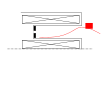
\includegraphics[width=\defaultwidth]{bshape}
    \caption{Usual shape of the axial profile of the radial magnetic field on the centerline of the channel.}
    \label{fig-bshape}
  \end{figure}


\section{HET operating principle}
% \addcontentsline{toc}{subsection}{HET operating principle}


  The operation principle of a \ac{HET} is rather simple.
  The objective is to ionize the propellant and impose an axial electric field to accelerate the ions.

  \paragraph{Ionization\\}
  The propellant, usually xenon, is ionized by electron-impact.
  The ionization energy needed is $\mathcal{E}_{\rm Xe, iz} = 12.13 \,\volt$, which corresponds to an electron velocity of $2000\,\kilo\meter\per\second$.
  Due to the low pressure (around $\sn{1}{-4}$ Pa), the mean free path of the electrons is larger than the chamber size.
  In consequence, a magnetic field is imposed in order to trap the electrons in a cyclotron motion.
  It increases the residence time of the electrons, thus promotes  ionization.
  In average in a well designed \ac{HET}, 90\% of the propellant is ionized.

  \paragraph{Acceleration\\}
  The potential difference  between the anode and the cathode is used to accelerate the ions outside of the chamber and create the thrust.
  Because the magnetic field slows the electrons down, the plasma resistivity increases in the region where the magnetic field amplitude is large.
  Hence, the axial profile of the magnitude of the axial electric field presents a maximum close to the maximum of the magnetic field.
  While the typical voltage difference is $U_d=300\,\volt$, the maximum electric field can be of the order of $30\,\kilo\volt\per\meter$ \citep{gawron2008}.

  \paragraph{Ionization and Acceleration regions overlap\\}
  \Cref{fig-zones} shows an illustration of the usual axial profiles of the ionization and the electric and magnetic fields.
  As the magnetic field governs both the ionization and the acceleration regions, it is challenging to obtain a clear separation between the two regions.
  However, if ionization happens in the acceleration region, the newly created ions will not be accelerated at their maximum velocity, hence resulting in a loss compared to the maximum theoretical thrust.
  The theoretical maximum speed is, by conservation of the total energy of the ion
  \begin{equation} \label{eq-vmaxtheo}
    v_{\rm ex, max} = \sqrt{ \frac{2 e U_d}{m_i} } \sim 31 \,\kilo\meter\per\second
  \end{equation}
  with $m_i = 131 \,\atomicmass$ for xenon and $U_d=300\,\volt$.
 \nomenclature[Q]{\ensuremath{ \atomicmass}}{ Atomic mass, $1\, \atomicmass \simeq \sn{1.66}{-27} \,\kilo\gram$}
 \nomenclature[P]{\ensuremath{ U_d}}{ Discharge voltage}

  \begin{figure}[hbt]
    \centering
    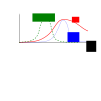
\includegraphics[width=\defaultwidth]{zones}
    \caption{Illustration of the usual axial profiles of the ionization and axial electric field amplitudes compared to the radial magnetic field amplitude.}
    \label{fig-zones}
  \end{figure}

  The thruster efficiency, in the usual configuration, is governed by its magnetic field topology.
  Hence, it can be tough to find the best topology that will optimize the ionization and the location of the ionization and acceleration regions.
  Some concepts of double stage \ac{HET} have been proposed to decouple the two phenomena to control them independently and are still under study \citep{dubois2018}.
  
  % However, the preliminary results are not as satisfactory as expected. 
  % \inlinenote{Add referecne here}
  % Moreover, the double-stage system needs more parts and power sources, resulting in a more complicated system.

  
  \section{Instabilities present in the \acs{HET} }
  \label{sec-physics}
  % \addcontentsline{toc}{subsection}{Instabilities present in the \acs{HET}}

  The \ac{HET}s are subject to numerous plasma oscillations, over a broad range of frequencies \citep{boeuf2017,choueiri2001}.
  The most important ones are\string:
  \begin{enumerate}
    \item Low frequency (10-20\,\kilo\hertz) ionization oscillations, usually referred to as breathing mode,
    \item Azimuthal low frequency rotating spokes, also in the \kilo\hertz{} range,
    \item Axial ion transit time oscillations, of the order of 100-500 \kilo\hertz,
    \item Azimuthal fast oscillations, of frequency of the order of the ion plasma frequency.
  \end{enumerate} 

  \paragraph{1. Breathing mode\\}
  The breathing mode is relatively understood \citep{boeuf1998,barral2009,hara2014}.
  Indeed, a simple predator-prey model of two equations is enough to obtain qualitatively the observed behavior.
  It is related to the idea that when the ionization is important, the neutral atom density decreases, reducing the ionization.
  Hence, the plasma density decreases, allowing the neutral density to rise again until the ionization grows up again.
  

  \paragraph{2. Rotating spokes\\}
  Experimental measurements with segmented anode \citep{ellison2012,mcdonald2011} seem to indicate that rotating spokes are present in the anode region.
  Their physical origins are less understood, as they were first attributed to ionization \citep{janes1966} but were later related to Simon-Hoh instability, and they were observed in \ac{PIC} simulations even with neglecting ionization \citep{carlsson2018}.
  However, in recent experiments, the presence of spokes did not seem to affect the \ac{HET} performances \citep{boeuf2017}.

  \paragraph{3. Transit time instability\\}
  Transit time instability has been predicted and observed in analytical and numerical models, respectively \citep{barral2005,boeuf2018}.
  Experimental studies of these instabilities are rather scarce, and it is only recently that time-resolved Laser-Induced Fluorescence measurements of the local ion velocity distribution function have confirmed the presence of this instability in a Hall thruster \citep{vaudolon2015}.
  This oscillation could reduce the performance of the thruster by increasing the overlap between the acceleration and ionization regions \citep{boeuf2018}.

  \paragraph{4. High-frequency azimuthal oscillations\\}
  These oscillations were first observed in \ac{PIC} simulations \citep{adam2004,ducrocq2006,adam2008a,heron2013} before being witnessed by electron Thomson scattering \citep{tsikata2009a,tsikata2009,tsikata2013}.
  They are essential, as they enhance the electron transport in the axial direction \citep{adam2004,lafleur2016a}.
  They are further described in the next section.

% !TEX root=/home/tavant/these/manuscript/src/manuscript.tex

\section*{Scientific challenges of the HETs}
\addcontentsline{toc}{section}{Scientific challenges of the HETs}

The scientific challenges are the key phenomena not understood enough that prevent the industrial development of \ac{HET}s.

\subsection*{Cross field transport of the elections}
\addcontentsline{toc}{subsection}{Cross field transport of the elections}

  \label{sec-mob}
  As a first approximation, the electrons are supposed frozen by the magnetic field.
  However, they can present a so-called cross-field transport.
  For instance, because of collisions, the electrons can move from one magnetic line to another.
  This leads to a transport in the direction of the electric field.
  
  This transport can be expressed considering the electron momentum conservation equation \citep{lafleur2016a}\string:
  \begin{equation} \label{eq-elec_momentum_mobility}
    \partial_t(m_e n_e \vect{v}_{de}) + \grad \cdot (m_e n_e  \vect{v}_{de} \vect{v}_{de}) = q_e n_e ( \vect{E} + \vect{v}_{de} \times \vect{B}) - \grad \cdot \vect{\Pi}_e - m_e \nu_m n_e \vect{v}_{de},
  \end{equation}
  where $m_e, q_e$, $n_e$, $\vect{v}_{de}$ and $\vect{\Pi}_e $ are the electron mass, charge, density, drift velocity and pressure tensor, and $\nu_m$ is the electron-neutral momentum transfer collision frequency.
  Ignoring the electron inertia and the pressure term, and with $\vect{B} = B_0 \vect{e}_r$, we can write the balance equation projected on the axial and azimuthal direction
  \begin{equation} \label{eq-elec_momentum_mobility2}
  \begin{cases}
    0 =  n_e E_z - n_e v_{de{\theta}} B_0 - \frac{m_e}{q_e} \nu_m n_e v_{dez}\\
    0 =  n_e E_{\theta} -  n_e v_{dez} B_0 - \frac{m_e}{q_e} \nu_m n_e v_{de{\theta}}
  \end{cases}
  \end{equation}
  Supposing that there is no electric field in the azimuthal direction ($E_{\theta}=0$),  we can combine the two equations of \cref{eq-elec_momentum_mobility2} and have \citep{chen2006,meezan2001}
  \begin{equation} \label{eq-mobility}
    \mobcla = \frac{n_e v_{dez}}{n_e E_z} = \frac{ \frac{\norm{q}}{m \nu_m}}{1 + \frac{\oce^2}{\nu_m}}
  \end{equation}
  with $\oce= \frac{\norm{q}B_0}{m}$ the cyclotron frequency.
  
  
  However, it has been observed in experiments by \citet{meezan2001} that the electron cross-field transport in the axial direction of the \ac{HET} is higher than $\mobcla$.
  Different phenomena have been proposed to explain the origin of this \emph{anomalous} transport.
  Two phenomena are supposed to be mainly responsible for this enhanced mobility \citep{croes2017}\string: the azimuthal instability and the near wall mobility due to electron emission.
  A significant part of the work of this Ph.D. thesis concerns the quantitative comparison of the relative importance of the two phenomena.

  
  \subsection*{Electron drift and azimuthal instability in the HETs}
  \addcontentsline{toc}{subsection}{Electron drift and azimuthal instability in the HETs}

  The axial electric field $E$ and the radial magnetic field $B$ induces an azimuthal $E\times B$ drift of the electrons.
  The drift velocity $v_{\rm d, ExB}$ is 
  \begin{equation} \label{eq-exbdrift}
    v_{\rm d, ExB} = \bigg\lvert \frac{\vect{E} \times \vect{B}}{B^2} \bigg\rvert = \frac{E}{B} \sim \sn{1.5}{6} \,\meter\per\second
  \end{equation}
  Because of their large mass, the ions are not significantly affected by the magnetic field, hence they do not drift azimuthally.
  As a consequence, there is a significant difference between the movement of electrons and ions in the azimuthal direction.

  This drift of electrons relative to the ions leads to instability in the azimuthal directions.
  Because the drift is perpendicular to the magnetic field, it is usually refereed as \ac{ECDI}.
  However, as it rises from an $E\times B$ drift, some authors use the name \ac{EDI}.
  In this thesis, we will use the name \ac{ECDI}.

  The actual nature of the \ac{ECDI} remains unclear\citep{boeuf2018}, as the \ac{ECDI} characteristic are very close to usual \ac{IAW}, and that experimental measurements are difficult to conducted in the range of parameter of interest.
  Hence, the community is still arguing about the actual nature of wave observed.
  A part of the work conducted during my theses concerns the study and characterization of the instabilities observed in the kinetic simulations.
  These instability are treated in \cref{ch-5}.
  
\subsection*{Plasma-wall interaction}
\addcontentsline{toc}{subsection}{Plasma-wall interaction}

  The ceramic wall closes the chamber in the radial directions.
  It have been observed in experiments that the nature of the wall can affect significantly the discharge behaviour \citep{gascon2003}.
  The main phenomenon hold responsible for this observation is the electron emission.
  As usually observed in bounded plasmas, a floating plasmas sheath forms between the plasma and the dielectric wall.
  The sheath confines the electrons in the plasma and accelerates the ions toward the walls.
  This allows to obtain a flux of electrons equals to the flux of ions, resulting in a charge conservation in the plasma, and a neutral flux, or also named zero-net current, to the surfaces.
  
  Due to the relatively high electron energy, the impact of a primary electron can lead to the emission of a secondary electrons \citep{barral2003a,villemant2018}.
  The probability of \ac{SEE} depends of the electron impact characteristics (energy, angle) but also of the material\string: some material are more emitting than others \citep{gascon2003}.
  Ion induced electron emission is much less likely to happen as the ions have a small energy of impact.
  In addition to the near wall conductivity discuss previously, these secondary electrons are accelerated toward the plasma by the sheath, and thus modify the plasma and the sheath properties.
  Their impacts on the electron temperature affects also the ionization rate, which is directly linked to the thruster efficiency.
  
  
  However, \citet{raitses2005} have observed that the current models of plasma-wall interactions with secondary electron emission cannot reproduce the electron temperature measurement experimentally.
  The kinetic phenomena have been proposed by \citet{sydorenko2007} to explain this discrepancy between the models and the experiments.
  This could explain the differences between the kinetic simulation results and the global models in \citet{croes2017}.   
    
  \vspace{1em}
  In addition to \ac{SEE}, the ion impact energy is large enough to erode the walls by sputtering.
  This erosion is large enough to be the main limitation of \ac{HET}s lifetime.
  While most aspects of the erosion are well understood, we observe the apparition or  patterns with a typical scale of the order of the millimeter on the eroded surfaces.
  The origin and the possible implications of these erosion striations remain open questions.
  

\subsection*{Three-dimensional physics of the HET}
\label{sec-3Dphi}
\addcontentsline{toc}{subsection}{Three-dimensional physics of the HET}

The description of the the physics governing the \ac{HET} really are three dimensional\string:
\begin{itemize}
  \item The plasma is accelerated in the axial direction by the electric field, and it is observed that the axial profile of the magnetic field is responsible for the performance of the thruster.
  \item The radial dimension is closed by the chamber walls. The walls are responsible for most of the plasma losses, both on the particle and energy balances.
  \item The electrons drifts in the azimuthal direction, leading to strong instabilities that affect the axial transport.
\end{itemize}

Consequently, when modeling or simulating an \ac{HET}, if one of the direction is not included, a part of the physics will be missing\string:
\begin{itemize}
  \item No axial direction\string: the ionization or the acceleration, as well as the plasma transport, are missing,
  \item No radial direction\string: the wall losses and interactions are missing,
  \item No azimuthal direction\string: the instability is missing, hence the electron cross-field transport is not well represented.
\end{itemize}

While \ac{3D}-simulations have recently been proposed, they uses scaling laws to simulate the system in a reasonable amount of time\citep{taccogna2019a}.
For instance, a reduced geometry is used in \citet{taccogna2018} or a reduced density is used in \citet{fubiani2018a}.
A \ac{3D} simulation at real scale is not yet accessible.
Hence, we need to be able to rely on \ac{1D} or \ac{2D} simulations.
Consequently, we have to take into account the missing physics or include a model of its effects on the system.

% !TEX root=/home/tavant/these/manuscript/src/manuscript.tex


\section*{Plasma models and simulations}
\label{sec-simulations}
\addcontentsline{toc}{section}{Plasma models and simulations}

Depending on the pressure, energy, and time scale, different models are more adapted to describe the plasma.
There are mainly two distinct models.
The first is the \emph{kinetic} description of the species of the plasma, via the Boltzmann equation.
The second uses a \emph{fluid} description of the species, by means of moments.
% 
% \begin{figure}[hbtp]
%   \centering
%   \includegraphics[width=\defaultwidth]{Chart}
%   \caption{}
%   \label{fig-chart}
% \end{figure}


\paragraph{Boltzmann equation \\}
The Boltzmann equation in \cref{eq-boltzmann} describes the evolution of the particles (atoms, ions and electrons) in the phase space.
The phase space is the set of each possible position $\vect{x}$ and velocity $\vect{v}$ that can be attained by a particle.
The evolutions in the phase space are due to forces, diffusion and collisions.

\begin{equation} \label{eq-boltzmann}
\deriv{f}{t}  + \vect{v} \cdot \grad_{\vect{x}} f + \vect{F} \cdot  \grad_{\vect{v}} f = \deriv{f}{t} \at{\rm coll}
\end{equation}
where $f$ is the distribution function of the particle at $\vect{x}, \vect{v}$, and $\deriv{f}{t}\mid_{\rm coll}$ denotes the effects of the collisions, $\grad$ is the gradient in both the positions (subscript $\vect{x}$) and the velocities (subscript $\vect{v}$)  and $\vect{F}$ is the force applied to the particle.
In the general electro-magnetic case,
\begin{equation*} \label{eq-forceEM}
  \vect{F} =  q \vect{E} + q \vect{v} \times \vect{B}
\end{equation*}
with $q$ the particle charge, $\vect{E}$ the electric field, and $\vect{B}$ the magnetic field.

\paragraph{Fluid equations \\}
The description in 7 dimensions (3 of space, 3 of velocity, and one of time) can complicate the resolution of the Boltzmann equation.
If the precise description of $f$ is not needed, we can instead use the first moments of \Cref{eq-boltzmann} on the velocity in order to obtain a set of simpler equations.

The first equation is obtained by integrating \cref{eq-boltzmann} over the velocity space, which gives
\begin{align}
    & \iiint_{\vect{v}}  \deriv{f}{t} d^3v &&+&& \iiint_{\vect{v}}  \vect{v} \cdot \grad_{\vect{x}} f  d^3v &&+&&  \iiint_{\vect{v}}  \vect{F} \cdot  \grad_{\vect{v}} f  d^3v && = && \iiint_{\vect{v}}  \deriv{f}{t} \at{\rm coll} \nonumber  \\ 
   \iff &  \deriv{n}{t} &&+&&  \grad_{\vect{x}}  \cdot  ( \vect{u} n) &&+&& 0 &&=&& S_{\rm iz}   \label{eq-conc}
\end{align} 
where $n=\iiint f d^3v$ is the density, $\vect{u} = \frac{1}{n} \iiint \vect{v} f d^3v$ is the mean velocity, and $S_{\rm iz}$ is the source term of particle due to ionization.
\Cref{eq-conc} is the continuity equation for a given species.

In the similar fashion, integrating the Boltzmann equation times the velocity and the kinetic energy gives the momentum conservation equation and the energy conservation equation, respectively.
This set of equation is simpler to approach, although it relies on more hypotheses.

One of them is the closure of the system.
Indeed, the continuity equation describes the evolution of the density $n$ but needs the mean velocity $\vect{u}$.
However, the velocity is described by the momentum conservation equation that need the temperature $T$, and so on.
In order to close the system, one has to make a hypotheses on the higher moment of the distribution function.
A usual closure is the isothermal hypotheses, that fix the temperature. 
Hence, the energy conservation equation is not needed.
Other closures possibles are the adiabatic hypotheses (no heath flux, the \nth{3} moment of $f$), the polytropic law linking the evolution of $n$ with $T$, or the Fourier law for heat diffusion.
% \inlinenote{Should we write the closes as equations ? $q = 0$, $T_e n_e ^{a}=cst$, etc. ?}


\subsection*{Plasma simulation models} \label{subsec-simulations}
As there are two different models to describe the plasma, there are two different simulation approaches \string: the fluid simulations and the kinetic simulations.
The fluid simulations solve the moments of the distribution function (the density, mean velocity and usually the temperature of the species), and the electromagnetic fields.
Depending of the conditions, the system of equation can be simplified before resolution.
In electrodynamic conditions, mainly for space plasmas and fusion, the Maxwell equations are coupled to the fluid equations leading to magnetohydrodynamics (MHD).
In the case of electrostatic conditions, as it is usual for Low Temperature plasmas, the Poisson equation is coupled to the fluid equations.
In most of low-temperature plasma, the plasma in quasi-neutral except in small regions as plasma sheaths close to walls.
It is also common to neglect inertia terms and assume a steady state in the momentum equations, leading to the drift-diffusion approximation
The fluid equations can be solved in \ac{3D}, \ac{2D} or \ac{1D} for space.
In low dimension model, the effects of the missing dimensions is usually added, for instance in the source terms as done by \citet{barral2003a}.The plasma is the state of matter in which atoms are ionized.


\vspace{1em}
However, some phenomena can only be described via the knowledge of the distribution function.
An example of such phenomena is the particle-wave interaction, as the Landau Damping \citep{landau1945,malmberg1964} or the plasma-beam instability \citep{filippychev1990}, for which the gradient of the distribution function in the velocity space is important.
In contrast to the fluid descriptions, \emph{kinetic} simulations solve for the distribution function for both position and velocities.
Two approaches are usually used for kinetic simulations\string:
\begin{itemize}
  \item The \ac{DK} model, that discretize \Cref{eq-boltzmann} in the full phase space.
  \item The \ac{PIC} model, which uses an ensemble of particles to discretize the distribution function.
\end{itemize} 
While the \ac{DK} simulations use an Eulerian description of the distribution function, we can see the \ac{PIC} simulations as a Lagrangian approach.
The \ac{DK} simulations can theoretically better describe the plasma, mostly because there is less numerical noise and we can model binary collision more easily, especially Coulomb collisions.
On the other hand, \ac{PIC} simulations are much more simpler to develop on both a mathematical and a computation perspective.
For instance, the kinetic effect of electron emission have been recently studied using \ac{DK} simulation by \citet{cagas2019}, while it has been done since the last century in \ac{PIC} simulations \citep{boswell1988}.



% \input{Context/6_LPPic}
% !TEX root=/home/tavant/these/manuscript/src/manuscript.tex

\section{Problem statement and outline of the thesis}
\label{sec-problematic}
% \addcontentsline{toc}{section}{Problematic of the thesis}

My thesis takes part of the collaboration between Safran Aircraft Engines and the Laboratory of Plasma Physics, whose objective is to study the fundamental physics governing the \ac{HET}, in the prospect of accelerating the developments of the next generations of thrusters.
I mainly focused on the electron transport and the plasma-wall interaction,
both aspects requiring the use of kinetic tools.

Indeed, the electron transport is affected by instabilities that can only be described by kinetic models \citep{adam2008a,lafleur2016a}.
Furthermore, the plasma-wall interaction is also affected by kinetic effects, both regarding the electron emission induced by electron impact \citep{barral2003a,raitses2011,sydorenko2006} and the wall erosion by ion impact sputtering.
Relatively few highly parallelized simulation codes  have been developed, that could allow parametric studies.
But the ever-increasing computational power available allows larger simulations to be conducted.
Thus, a significant part of my work involves the development of a highly efficient \ac{PIC} simulation code, with all of the technical difficulties related to it.
The simulation code is then used to proceed to several parametric studies, that I used to derive reliable low-dimensional models that could be used to derive new engineering development tools.


\vspace{1em}
In \cref{ch-1}, we introduce \LPPic, the primary simulation model used in this work, with an emphasis on the axial convection of the particles and the plasma-wall interaction.
\cref{ch-5} focus on the azimuthal instability observed in the simulation and compares it to the dispersion relation.
\cref{ch-2} presents the results of a parametric study investigating the wall effect.
In \cref{ch-3,ch-4}, we modify the sheath model in order to reproduce the \ac{PIC} simulation results.
\cref{ch-3} focuses on a simplified \ac{1D} simulation to study the electron state law, while \cref{ch-4} continues the same model by including the secondary electron emission.
While the majority of the work studied the \ac{2D} radial and azimuthal simulation, we end by studying the radial direction in a \ac{2D} axial and azimuthal simulation in \cref{ch-6}.


% \acresetall

\let\leftmark=\oldleftmark
\let\rightmark=\oldrightmark

\renewcommand\thechapter\oldthechapter
\renewcommand\chaptername{Chapter}

% !TEX root=/home/tavant/these/manuscript/src/manuscript.tex




\chapter{Particle-In-Cell simulations of Hall Effect Thrusters}
\label{ch-1}
Structure :

{\bf Particle in Cell simulations} 20 pages
\begin{zzz}
  
  1.1 The HET
  1.2 Elements of the 2D PIC-MCC simulations

  1.3 Numerical implementation

  1.4 R-theta simulation: hypotheses
  
  1.5 focus on  Dielectrics : Poisson equation 

  1.6 Axial convection model
  
  1.7 Conclusion
\end{zzz}
\inlinenote{Is missing a part of the HET physics. Like the Boeuf Tutorial. }
\inlinenote{Missing SEE }

The \ac{HET} has been studied since its first designs int he 1960's.
However, the physical processes the govern its behaviour stay ill-understood.
For most of them, as the electron cross field mobility or the plasma-surface interactions, kinetic informations are needed.


The next section present the basics of the \ac{PIC} - \ac{MCC} simulations, and the simulations code \LPPic that is develop at \ac{LPP}.


\inlinenote{add SEE models, discussions concerning the choice we did, a.s.o.}
 
% !TEX root=/home/tavant/these/manuscript/src/manuscript.tex


% !TEX root=/home/tavant/these/manuscript/src/manuscript.tex

\section{Elements of the 2D PIC-MCC simulations}
  \label{sec-elements}
  \subsection{Principe of the PIC simulations}

    The \ac{PIC} simulation models particles moving freely on a grid.
    The grid is used to compute the electric field, in the electrostatic approximation by solving the Poisson equation

    \begin{equation}
      \label{eq-poisson}
      \Delta \phi = - \frac{\rho}{\epsilon_0}
    \end{equation}

    where $\phi$ is the electric potential, $\rho$ is the charge density, and $\epsilon_0$ the vacuum permittivity.
    If the electrostatic approximation is not correct, one need to solve the Maxwell equations.

    The particles move following the Lorenz forces
    \begin{equation}
      \label{eq-Lor}
      m \vec{a} = q \vect{E} + q \vec{v} \times \vec{B}
    \end{equation}
    with $m$ and $q$ the particle mass and electric charge respectively.
    The numerical particles followed in the simulations correspond to $q_f$ physical particles, with
    \begin{equation}
      q_f = \frac{n V}{\Npc}
    \end{equation}
    with $n$ the particle density, $V$ the volume of a cell, and $\Npc$ the number of numerical particle in a cell.
    A large enough number of particle is needed in order to obtain physical results.
    Indeed, insufficient number of particles leads to numerical heating \cite{ueda1994}.
    Usually, a minimum of 100 particles per cell are used, but recent results seem to encourage to use more particle \cite{janhunen2018}.

  \subsection{Monte Carlo collisions}

    In \ac{PIC} simulations, collisions between charged and neutral particles can be modeled by binary collision, but this approach is computationally costly.
    Instead, a Monte-Carlo algorithm can be used \cite{vahedi1995}.
    This approach is very efficient, and allow scattering, momentum transfer and ionization to be consistently modeled.
    The propellant used in \ac{HET} usually is \ac{Xe}, even if the recent constellation Starlink uses \ac{Kr}.
    The cross sections used for modeling \ac{Xe} or other gases collisions are taken from the {\sc LXCat} database project \cite{LXCat_web}.
    Except if otherwise stated, the elastic, inelastic scattering and ionization reactions listed in \cref{tab-reactXe} are used.
    The cross section values are summarised in \cref{fig-xexsection}.

    \begin{table}[hbtp]
      \ra{1.3}
      \centering
      \caption{Reactions for xenon used in the PIC simulations}
      \label{tab-reactXe}
      \begin{tabular}{@{}lll@{}}  \toprule
        Reaction & Threshold & Reference\\ \midrule
        {\it Elastic scattering} & &\\
        e + Xe = e + Xe   & --   & \cite{Lxcat_Xe,Lxcat_Xe2} \\
        {\it Excitation} & &\\
        e + Xe = e + Xe$^*$   & 8.315eV   & \cite{Lxcat_Xe,Lxcat_Xe2} \\
        e + Xe = e + Xe$^*$   & 9.447eV   & \cite{Lxcat_Xe,Lxcat_Xe2} \\
        e + Xe = e + Xe$^*$   & 9.917eV   & \cite{Lxcat_Xe,Lxcat_Xe2} \\
        e + Xe = e + Xe$^*$   & 11.7eV    & \cite{Lxcat_Xe,Lxcat_Xe2} \\
        {\it Ionization} & &\\
        e + Xe = e + Xe$^+$   & 8.315eV   & \cite{Lxcat_Xe,Lxcat_Xe2} \\
        \bottomrule
      \end{tabular}
    \end{table}



    \begin{figure}[hbtp]
      \centering
      \includegraphics[width=\defaultwidth]{figure/xenon_cross_section.pdf}
      \caption{Cross section values used in the Monte Carlo procedure \cite{Lxcat_Xe,Lxcat_Xe2}.}
      \label{fig-xexsection}
    \end{figure}


\section{Numerical implementation of the Particle in cell simulation}

  \LPPic is an explicit electrostatic \ac{PIC}-\ac{MCC} simulation code.
  Every time-steps, the simulation loop presented in \cref{fig-picloop} is computed.
  The different steps constituting the PIC-loop are described in the next subsections.
  \begin{figure}[hbtp]
    \centering
    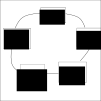
\includegraphics{picloop.png}
    \caption{\ac{PIC}-\ac{MCC} loop executed every time steps.}
    \label{fig-picloop}
  \end{figure}

  \subsection{Data used}
    In the \ac{PIC} simulations, there are two kind of data used\string:
    \begin{itemize}
      \item Particles (electron, ions, neutral can be followed as well but not in \LPPic)
      \item Mesh, also named fields (densities, electric and magnetic fields, and so on)
    \end{itemize}

    \paragraph{Particles\\}
    For each particles, are known its position $\vec{x}$ and its velocity $\vec{v}$.
    In most \ac{PIC}-\ac{MCC} simulations, the 3 directions of the velocity vector are followed in order to in order to take into account scattering.
    It is abbreviated as \acs{3V}.
    
    \paragraph{Fields\\}
    The fields are defined at the center of each cell of the mesh.
    The charge density $\rho$ is computed by depositing the particle on the mesh, using the Cloud-in-cell model \cite{birdsall1991}.
    The electric field at the position of the particle is also obtain by bi-linear interpolation.
    The mesh dimension defines the dimension of the simulation.
    It is usual to find \acs{1D}\acs{3V} or \acs{2D}\acs{3V} \ac{PIC} simulations, for particles with 3 directions on the velocity but 1 (or 2) dimensions in space.

    \subsection{Particle pusher}
    The interaction of the movement equation \cref{eq-Lor} is different for magnetized and non-magnetized particles.

    For non-magnetized particles, we use the leapfrog scheme \cite{birdsall1991}
    \begin{align}\label{eq-leapfrog}
      \vect{v}^t &= \vect{v}^{t-1} + \frac{q}{m} \vect{E} \dt, \\
      \vect{x}^t &= \vect{x}^{t-1} + \vect{v}^t \dt,
    \end{align}
    with the superscript $t$ designing the time step, $q$ and $m$ the particle electric charge and mass, $\vect{E}$ the electric field at the particle position, and \dt the time step duration.

    It is important to note that the leapfrog induces a shift of $\frac{\dt}{2}$ between the position and the velocity, as illustrated in \cref{fig-leapfrog}.
    \begin{figure}[hbtp]
      \centering
      \includegraphics[width=\defaultwidth]{leapfrog.png}
      \caption{Illustration of the shift between the particle velocity and position.}
      \label{fig-leapfrog}
    \end{figure}
    This shift can leads to erroneous diagnostics when computing moments of the particles distribution.
    For instance, the mean velocity of an ensemble of $N$ particle at the instant $t$ is computed as\string:
    \begin{equation} \label{eq-meanv}
      \mean{\vect{v}}^t = \frac{1}{N} \sum_i^N \lp \vect{v_i}^t + \frac{q}{m} \vect{E_i} \frac{\dt}{2} \rp.
    \end{equation}
    Other moments like the mean energy or heat flux follow the same correction.
    We can see that the error between $\mean{\vect{v}}$ defined above and
    $$ \tilde{\vect{v}} = \frac{1}{N} \sum_i^N  \vect{v_i}^t $$
    is
    $$ \mean{\vect{v}} - \tilde{\vect{v}} =\frac{q \dt}{2 m}  \frac{1}{N}  \sum_i^N  \vect{E_i} .$$
    Hence, the error in the diagnostic is larger in the region of large electric field (as in the sheaths).

    \paragraph{Magnetized particles}
    For magnetized particles, we use a modification of the leapfrog algorithm proposed by Boris \cite{boris1970}.
    It correspond to an operator splitting between the electrostatic acceleration and the magnetic rotation.
    This splitting is describe below\string:

    \begin{enumerate}
      \item accelerate the particle during $\frac{\dt}{2}$ \string: $\vect{v}^{t-\frac{\dt}{2}} = \vect{v}^{t-1} + \frac{q}{m} \vect{E} \frac{\dt}{2}$
      \item rotate the particle velocity with the magnetic field
      \item accelerate the particle during $\frac{\dt}{2}$ \string: $\vect{v}^t = \vect{v}^{t-\frac{\dt}{2}} + \frac{q}{m} \vect{E} \frac{\dt}{2}$
    \end{enumerate}


  \subsection{Poisson equation solver}
  \label{subsec-poissonintro}

    The Poisson equation \cref{eq-poisson} is an elliptic equation.
    We can directly discretize the differential operator by finite volume on the cell mesh.
    The formal discretization is develop in \cref{sec-diel}, but a short summary is given here.

    In \ac{1D}, the obtained linear system is tridiagnonal.
    It can be solve directly using {\sc Thomas} algorithm, which simply stores the Gauss elimination's coefficient.
    In \ac{2D}, the linear system is pentadiagonal.
    A direct solver, like the $LU$ decomposition, would require a large amount a memory to store the factorisation matrices.
    On the other hand, as the time step is usually small in \ac{PIC} simulation, we expect the plasma potential $\phi$ not to change rapidly.
    Hence, an iterative solver using the previous solution as initial guess seems more reasonable fro both the memory storage and the computational time.

    In practice, we uses {\sc Hypre}'s multigrid solver to solve Poisson equation in \ac{2D} in \LPPic.

% !TEX root=/home/tavant/these/manuscript/src/manuscript.tex

\section{Bidimentionnal simulation of an Hall Effect Thruster}


\subsection{The Hall effect Thruster }

The \ac{HET} is an electrostatic electrical propulsion system accelerating ions by the mean of an imposed voltage difference.

We can summarize its composition by four parts:
\begin{enumerate}
  \item The annular chamber.
  \item The injecting anode
  \item The cathode
  \item The magnetic circuit
\end{enumerate}

\paragraph{The chamber} has an annular shape.
It is open closed at the anode side, and kept open at the other side.
The walls are usually constituted by a ceramic, usually \ac{BNSiO2}.
The material needs to be resistant to erosion by ion impact sputtering.
But changing the material is also known to affects the discharge behaviour.
The usually supposed phenomena for this impact is the secondary electron emission yield that is a function of the material nature.


\paragraph{The anode} is at the bottom of the chamber.
The anode voltage is imposed to a few hundred volts.
Usually, the neutral gas injection is made by the anode itself.
The mass flow rate is of the order of a flew mg/s.

\paragraph{The cathode} is outside of the chamber.
It is grounded, and injects electrons for two reasons:
\begin{itemize}
  \item most of the electrons ($\sim 90 \%$) are used to neutralize the ion flux, for both allowing the ions to leave the thruster and avoid charging of the spacecraft.
  \item some of the electrons are attracted by the anode, hence entering the chamber and allowing the plasma discharge and switch and remain on.
\end{itemize}

% !TEX root=/home/tavant/these/manuscript/src/manuscript.tex

\section{Dielectrics boundary condition}
  \label{sec-diel}

  \Cref{fig-2dschemat} shows the simulation of the radial-azimuthal domain with metallic grounded walls.
  \Cref{fig-2D} illustrates the configuration in the radial-azimuthal planehighlighting the more realistic radial boundary conditions.
  The plasma is bounded in the radial direction by dielectric layers isolating the magnetic circuit.
  The magnetic circuit can be considered electrically grounded.

  The particles are absorbed when touching the dielectric wall, and we suppose an infinite residence time.
  Hence, we obtain a surface charge $\sigma$ at a time $t$ with
  \begin{equation} \label{eq-sigmaintegrate}
    \sigma(t) = e \int_0^t (J_i - J_e) dt
  \end{equation}
  with $J_i$ and $J_e$ the ion and electron flux respectively and $e$ is the elementary charge and supposing that there is no surface charge at the interface at the beginning.

  \begin{figure}[hbtp]
    \centering
    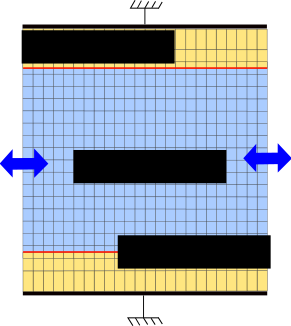
\includegraphics[width=\defaultwidth]{2D_diel_Rtheta}
    \caption{Schematic representation of the dielectric layers between the plasma in the \ac{2D} radial-azimuthal plan. Are present the dielectric in yellow, the plasma in blue, the surface charges in red and the grounded magnetic circuit in black.}
    \label{fig-2D}
  \end{figure}


  A common approach is to suppose that the electric field inside the dielectric is zero \citep{taccogna2019}. 
  Using Gauss theorem, we obtain a Neumann boundary condition at the plasma-wall interface for the potential
  \begin{equation} \label{eq-gauss}
    \norm{\partial_r \phi} = \frac{\norm{\sigma}}{\epsilon_0}
  \end{equation}
  with $\sigma$ the surface charge and $\epsilon_0$ the vacuum permittivity.
  However, the electric field in a dielectric material is not zero, but depends on the global system.
  Hence, in order to model correctly the dielectric wall of the \ac{HET}, we choose to include the whole dielectric layers inside of the simulation domain.

  In this section, we derive the discretization of the Poisson equation with non-uniform permittivity in the \ac{2D} radial azimuthal plane using the finite volume approach.


  \subsection{Non-uniform mesh}

    In the dielectric layers, there is no particle nor charge.
    Hence, the numerical constraints on the cell size are not applicable, and the cell size can be increased.
    In order to reduce the cell size difference between two neighbouring cells, we use an exponential growth of the cell size in the radial direction.
    The cell size in the azimuthal direction $\dy$ is kept constant.
    The resulting non-uniform mesh can be seen in \cref{fig-2D}.


  \subsection{Poisson equation discretization}


  The dielectric permittivity is $\epsilon= \epsr \epsilon_0$ with $\epsr$ the relative permittivity of the dielectric.

  The Poisson equation with not-constant permittivity is
  \begin{equation} \label{eq-poissondiel}
    \grad \cdot \epsilon \grad \phi = \rho
  \end{equation}
  with $\rho$ the charge density.
  We note $\vect{D}=\epsilon \vect{E} = \epsilon \grad \phi$ the electric flux.

  \Cref{fig-decompo1} shows the Cartesian decomposition of the \ac{2D} domain.
  The cell $(i,j)$ has four direct neighbours\string:
  \begin{itemize}
    \item the east $E$ in $(i+1,j)$
    \item the west $W$ in $(i-1, j)$
    \item the north $N$ in $(i, j+1)$
    \item the south $S$ in $(i, j-1)$
  \end{itemize}
  The cell dimensions are $\dx_{i,j}$ and $\dy_{i,j}$, and $\V=\dx_{i,j} \dy_{i,j}$ is the cell volume.
  As the mesh is Cartesian, we have for a given $j$ $\dx_{i,j} = cst$ for all $i$. Hence, we note $\dx_{i,j} = d_i$ and $\dy_{i,j} = d_j$

  The boundaries are noted $S^s_{i,j}$ with $s=E,W,N$ or $S$.
  We can see that $S^W_{i,j}=S^E_{i-1,j}$, and the same goes for the other borders.
  We note $\C = S^E_{i,j} \cup S^W_{i,j} \cup S^N_{i,j} \cup S^S_{i,j}$ the cell surface boundary.
  The center of the cell is located in $i,j$ and the borders are located in $i\pm 1/2$ in the East-West direction and $j\pm 1/2$ in the North-Sourth direction.
  \begin{figure}[hbt]
    \centering
    \includegraphics[width=\defaultwidth]{discrect1.pdf}
    \caption{Illustration of the Cartesian decomposition of the \ac{2D} domain}
    \label{fig-decompo1}
  \end{figure}


  \subsection{Poisson equation discretization}

    We start by positioning the plasma-dielectric interface on the surface between two cells.
    This means that the permittivity $\epsilon = \epsilon_0 \epsr$ is  constant over a cell.
    In order to discretize the Poisson equation, we integrate \cref{eq-poissondiel} over the cell volume

    \begin{equation}
    \int_{\V} - \grad \cdot (\epsilon \grad \phi) dv= \int_{\V} \rho dv.
    \end{equation}
    Using Gauss-Ostrogradsky theorem, we obtain
    \begin{equation}
    \oint_{\C} ( - \epsilon \grad \phi) \cdot \vect{n} dS = Q_{tot} =  \V \bar{\rho},
    \end{equation}
    with $\vect{n}$ the normal vector directed outward, $Q_{tot}$ is the total charge of the cell and $\bar{\rho}$ is the mean value of $\rho$ in the cell.
    We can decompose the integration over the cell boundary with the four surfaces $S^s_{i,j}$ as
    \begin{equation}
      \label{eq-poissonsum}
    \oint_{\C} (-\epsilon \grad \phi) \cdot \vect{n} dS = \sum_{k\in(E,W,N,S)} S^k_{i,j} \vect{D}^k_{i,j} \cdot \vect{n}
    \end{equation}
    with $\vect{D}^k_{i,j}$ the flux through the surface $k$ of the cell $(i,j)$.


    \paragraph*{Electric flux \\}
    Let us define the electric flux through the East border  $\vect{D}^E_{i,j}$.
    We suppose there is no surface charges on $S^E$.
    We can hence write the electric flux as
    \begin{align} \label{eq-flux1}
      \vect{D}^E_{i,j} \cdot \vect{n} &= \epsilon_{i,j} E_{x, i+1/2,j}^-\\
                                      &= - \epsilon_{i,j} \frac{\phi_{i+1/2,j} - \phi_{i,j}}{d_i/2},
    \end{align}
    with an off-center discretization of the electric field.

    Using the Gauss's law without charges
    \begin{equation} \label{eq-gausslaw}
      \epsilon_{i,j}E_{x, i+1/2,j}^- - \epsilon_{i+1,j}E_{x, i+1/2,j}^+ =0,
    \end{equation}
    we have
    \begin{equation}
      \epsilon_{i,j} \frac{\phi_{i+1/2,j} - \phi_{i,j}}{d_i/2} = \epsilon_{i+1,j} \frac{\phi_{i+1,j} - \phi_{i+1/2,j}}{d_{i+1}/2}.
    \end{equation}
    Hence
    \begin{equation} \label{eq-phidemi1}
      \phi_{i+1/2,j} = \frac{\epsilon_{i,j} d_{i+1} \phi_{i,j} + \epsilon_{i+1,j} d_{i} \phi_{i+1,j} }{\epsilon_{i,j} d_{i+1} + \epsilon_{i+1,j} d_{i} },
    \end{equation}
    which corresponds to the usual discretization when $\epsilon$ and $d_i$ are both constant.
    Using \cref{eq-phidemi1} in \cref{eq-flux1} we obtain
    \begin{align}
      \label{eq-nosc}
    \vect{D}^E_{i,j} \cdot \vect{n} &=& 2\frac{\epsilon_{i,j}\epsilon_{i+1,j}}{\epsilon_{i,j}d_{i+1} + \epsilon_{i+1,j} d_i} (\phi_{i,j}-\phi_{i+1,j})
    &=& 2\epsilon_0 \frac{\epsr{i,j}\epsr{i+1,j}}{\epsr{i,j}d_{i+1} + \epsr{i+1,j} d_i} (\phi_{i,j}-\phi_{i+1,j})
    \end{align}

    We note $Q^E_{i,j} \equiv \frac{\epsilon_{i,j} \epsilon_{i+1,j}}{\epsilon_{i,j} d_{i+1} + \epsilon_{i+1,j} d_i}$.
    reproducing the same decomposition on the other borders, we obtain
    \begin{equation}
      \label{eq-descretPoisson1}
    S^E_{i,j} Q^E_{i,j} \phi_{i+1,j} + S^W_{i,j} Q^W_{i,j} \phi_{i-1,j} + S^N_{i,j} Q^N_{i,j} \phi_{i,j+1} + S^S_{i,j} Q^S_{i,j} \phi_{i,j-1} - Q^C_{i,j} \phi_{i,j} = - \V \bar{\rho_{i,j}}
    \end{equation}
    with
    \begin{center}
      $\begin{dcases}
     Q^E_{i,j} &= 2\frac{\epsilon_{i,j} \epsilon_{i+1,j}}{\epsilon_{i,j} d_{i+1} + \epsilon_{i+1,j} d_i} \\
     Q^W_{i,j} &= Q^E_{i-1,j} \\
     Q^N_{i,j} &= 2\frac{\epsilon_{i,j} \epsilon_{i,j+1}}{\epsilon_{i,j} d_{j+1} + \epsilon_{i,j+1} d_{j}}\\
     Q^S_{i,j} &= Q^N_{i-1,j} \\
     Q^C_{i,j} &= Q^E_{i,j}S^E_{i,j}+Q^W_{i,j}S^W_{i,j}+Q^N_{i,j}S^N_{i,j}+Q^S_{i,j}S^S_{i,j}
     \end{dcases}$
    \end{center}

    as well as $S^E_{i,j} = S^W_{i,j} =d_id_z, S^N_{i,j} = S^S_{i,j}= d_jd_z$ et $\V = d_jd_id_z$.
    We observe that the evolution of the relative permittivity and the cell size affects the coefficients to be used, but the system remains symmetric as we have $Q^S_{i,j} = Q^N_{i-1,j}$ and $ Q^W_{i,j} = Q^E_{i-1,j}$.
    
    A symmetric system is a linear system of equation $A \cdot X = B$  which matrix $A$ is equal to is transpose: $A = A^T$.
    It allows to reduce by a factor of two the memory needed to store the matrix.
    It also allows to use algorithm exploiting this aspect. For instance, the eigenvalues are real-valued, and the matrix factorisation only need to store one factor using Cholesky decomposition, which gives $A = L L^T$ with L an upper-triangular matrix. 

    \subsection{Including surfaces charges}
    Let's now considerer the presence of surface charges on the surface $S^E_{i,j}$.
    Gauss's law now reads
    \begin{equation} \label{eq-gausslawsc}
      -\epsilon_{i,j}E_{x, i+1/2,j}^- + \epsilon_{i+1,j}E_{x, i+1/2,j}^+ =\sigma^E,
    \end{equation}
    with $\sigma^E$ the surface charge on the surface.
    The surface charge is not taken into account when computing the total charge in a cell.
    Using the same discretization as before, we obtain
    \begin{equation}
    \epsilon_{i,j} \frac{\phi_{i+1/2,j} - \phi_{i,j}}{d_i/2} - \epsilon_{i+1,j} \frac{\phi_{i+1,j} - \phi_{i+1/2,j}}{d_{i+1}/2} = \sigma^E
    \end{equation}
    so that
    \begin{equation}
      \label{eq-phidemi}
    \phi_{i+1/2,j} = \frac{\epsilon_{i,j} d_{i+1} \phi_{i,j} + \epsilon_{i+1,j} d_{i} \phi_{i+1,j} }{\epsilon_{i,j} d_{i+1} + \epsilon_{i+1,j} d_{i} } + \frac{1}{2}\sigma^E \frac{d_i d_{i+1}}{\epsilon_{i,j} d_{i+1} + \epsilon_{i+1,j} d_{i}}
    \end{equation}
    hence
    \begin{align*}
    \vect{D}^E_{i,j} \cdot \vect{n} &= 2\frac{\epsilon_{i,j}\epsilon_{i+1,j}}{\epsilon_{i,j}d_{i+1} + \epsilon_{i+1,j} d_i} (\phi_{i,j}-\phi_{i+1,j}) - \sigma^E \frac{\epsilon_{i,j}d_{i+1}}{\epsilon_{i,j}d_{i+1}+\epsilon_{i+1,j}d_{i}}
    \end{align*}
    We obtain the same relation that \cref{eq-nosc} updated by $- \sigma^E \frac{\epsilon_{i,j}d_{i+1}}{\epsilon_{i,j}d_{i+1}+\epsilon_{i+1,j}d_{i}}$

    Hence, we finally obtain
    \begin{equation}
    S^E_{i,j} Q^E_{i,j} \phi_{i+1,j} + S^W_{i,j} Q^W_{i,j} \phi_{i-1,j} + S^N_{i,j} Q^N_{i,j} \phi_{i,j+1} + S^S_{i,j} Q^S_{i,j} \phi_{i,j-1} - Q^C_{i,j} \phi_{i,j} = - \V \bar{\rho_{i,j}} + Q^W_{\sigma} \sigma^W
    \end{equation}
    with $Q^W_{\sigma} =  S^W_{i,j} \frac{\epsilon_{i,j}d_{i-1}}{\epsilon_{i,j}d_{i-1}+\epsilon_{i-1,j}d_{i}}$.



  \subsection{Verifications}
    We verify the discretization by modeling a \ac{1D} capacitor.
    The relative permittivity of the dielectric inside the capacitor (from $x=0.4$ to $0.6$) is set to $\epsr = 8$, and a surface charge of  $\sigma = 8$~nC.cm$^{-2}$ is imposed on one side, and $-8$~nC.cm$^{-2}$ on the other side.
    The expected electric field in the capacitor using the infinite plane approximation is $E = \sigma/(\epsilon_0\epsr) = 1.15$~kV.mm$^{-1}$.

    \Cref{fig-surface} shows the electric field computed using the obtained decomposition.
    We see that we obtain the expected value for the electric field.


    \begin{figure}[hbtp]
      \label{fig-surface}
      \centering
      \includegraphics[width=\defaultwidth]{potential.pdf}
      \caption{Electric field of the capacitor configuration calculated by the Poisson solver in order to validate the discretization and the solver. }
    \end{figure}


  \subsection{Interface at the cell centre}
    In the previous section, we supposed that the plasma-dielectric dielectric boundary was at the interface between the cells.
    However, this means that the electric field close to the interface is unknown, as it is defined at the cell center.
    Moreover, the Dirichlet condition for the potential is better defined at the cell center, and for sake of simplicity, changing the boundary conditions should not change the particle domain.
    Hence, we chose to position the plasma-wall interface at the center of the cell.
    This means that the permittivity is not constant over a cell.

    Because the wall boundaries are only in the radial directions, we consider only an interface in the North-South direction.
    \Cref{fig-decompo2} shows the domain decomposition.
    The decomposition is the same as previously, except for the permittivity that can have two different values\string: one in the North half-plane${\epsr}_{, i,j}^n$ and another in the South half plane${\epsr}_{, i,j}^s$.

    \begin{figure}[hbt]
      \centering
      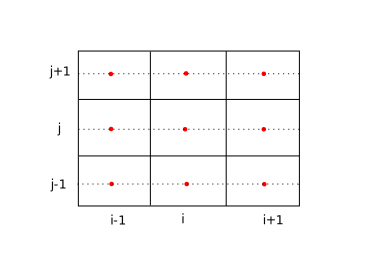
\includegraphics[width=\defaultwidth]{discrect2.pdf}
      \caption{Cartesian decomposition of the \ac{2D} domain. The dash lines represent discontinuities in the permittivity value.}
      \label{fig-decompo2}
    \end{figure}

    The discretization of the Poisson \cref{eq-poissonsum} is follows the same path as previously,except that the electric flux in equation in not constant any more, so that \cref{eq-poissonsum} becomes
    \begin{equation}
    \oint_{\C} (-\epsilon \grad \phi) \cdot \vect{n} dS = \sum_{k\in(E,W,N,S)} S^k_{i,j} <\vect{D}^k_{i,j} \cdot \vect{n}>.
    \end{equation}

    We can define
    \begin{align}
    <\vect{D}^E_{i,j} \cdot \vect{n} >&= \frac{1}{2} \epsilon_{i,j}^N E_{x, i+1/2,j}^- + \frac{1}{2} \epsilon_{i,j}^S E_{x, i+1/2,j}^-\\
     &= \frac{-1}{2} (\epsilon_{i,j}^N + \epsilon_{i,j}^S) \frac{\phi_{i+1/2,j} - \phi_{i,j}}{d_i/2}
     \label{eq-flux}
    \end{align}
    so that in the Est-West direction, the flux behave as if the cell permittivity is the mean of the North and South half plane$\epsilon_{i,j} = \frac{1}{2} (\epsilon_{i,j}^N + \epsilon_{i,j}^S)$.
    Hence, the rest of the computation is similar.
    For the boundary North and South, the permittivity is constant, hence there is no modification.
    Consequently, we obtain the discretization
    \begin{equation}
    S^E_{i,j} Q^E_{i,j} \phi_{i+1,j} + S^W_{i,j} Q^W_{i,j} \phi_{i-1,j} + S^N_{i,j} Q^N_{i,j} \phi_{i,j+1} + S^S_{i,j} Q^S_{i,j} \phi_{i,j-1} - Q^C_{i,j} \phi_{i,j} = - \V \bar{\rho_{i,j}}
    \label{eq-descretPoissoncentered}
    \end{equation}
    with
    \begin{center}
     $\begin{dcases}
     Q^E_{i,j} &= 2\frac{\epsilon_{i,j} \epsilon_{i+1,j}}{\epsilon_{i,j} d_{i+1} + \epsilon_{i+1,j} d_i} \\
     Q^W_{i,j} &= Q^E_{i-1,j} \\
     Q^N_{i,j} &= 2\frac{\epsilon_{i,j}^N \epsilon_{i,j+1}^S}{\epsilon_{i,j}^N d_{j+1} + \epsilon_{i,j+1}^S d_{j}}\\
     Q^S_{i,j} &= 2\frac{\epsilon_{i,j}^S \epsilon_{i,j-1}^N}{\epsilon_{i,j}^S d_{j+1} + \epsilon_{i,j-1}^N d_{j}} \\
     Q^C_{i,j} &= Q^E_{i,j}S^E_{i,j}+Q^W_{i,j}S^W_{i,j}+Q^N_{i,j}S^N_{i,j}+Q^S_{i,j}S^S_{i,j}
     \end{dcases}$
    \end{center}

    As well as $S^E_{i,j} = S^W_{i,j} =d_id_z, S^N_{i,j} = S^S_{i,j}= d_jd_z$ et $\V = d_jd_id_z$.
    Here, the system is no more symmetric.
    However, we can suppose that the only permittivity jump happens at the cell center, so that  $\epsilon_{i,j}^S = \epsilon_{i,j-1}^N$.
    Hence, $Q^N_{i,j} = 2\frac{\epsilon_{i,j}^N}{ d_{j+1} + d_{j}}$ and the system is symmetric.

  \subsection{Surface charges for centred interface}
    in the case of centered plasma-wall interface, we have surfaces charges at the center of the cell.
    Hence
    \begin{equation}
    \int_{\Omega_{i,j}} \rho dv = \Omega_{i,j}\bar{\rho} + S_{i,j}^N \sigma_{i,j}.
    \end{equation}
    The surface charges behave like volume charges.
    Hence, we obtain
    \begin{equation}
    S^E_{i,j} Q^E_{i,j} \phi_{i+1,j} + S^W_{i,j} Q^W_{i,j} \phi_{i-1,j} + S^N_{i,j} Q^N_{i,j} \phi_{i,j+1} + S^S_{i,j} Q^S_{i,j} \phi_{i,j-1} - Q^C_{i,j} \phi_{i,j} = - \V \bar{\rho_{i,j}} - S^N_{i,j} \sigma_{i,j}
    \end{equation}

    The discretization obtained for the plasma-wall interface cell-centred is very similar to the one obtained for the interface at the cell interface.
    However, it conserves the particle domain when the dielectric layer is not modeled and that Dirichlet conditions are applied, and the electric field at the plasma-wall interface is better defined.
    Hence, the cell-centred interface will be used.

    \inlinenote{Ajouter validation de la resolution}
    
  \subsection{Electric field computation}
  
  \subsection{Numerical resolution the Poisson equation}
  
  
% !TEX root=/home/tavant/these/manuscript/src/manuscript.tex

\section{Axial Convection model}
  \label{sec-reinjectionnoise}
  \inlinenote{Add the section about reinjection noise.}

  As introduce in the previous section, the \ac{2D} radial-azimuthal simulation do not model a priori the convection.

  \subsection{Lafleur's model of injection}

    \citet{lafleur2016a} proposed a way to model the axial convection of the particles in a \ac{1D} purely azimuthal simulation.
    \Cref{fig-Fake_1d_1} shows a schematic illustration of the model.
    The principle is as follow
    \begin{itemize}
      \item We set a finite axial length, noted $L_z$ on \cref{fig-Fake_1d_1}.
      \item We follow the positions of the particle in the axial direction $z$
      \item When a particle crosses the boundary, it is removed.
      \item A new particle is created
      \begin{itemize}
        \item at $z=0$ for the ions
        \item  at $z=L_z$ for the electrons
      \end{itemize}
    \end{itemize}

    We create a new particle in order to conserve the charge in the simulation.
    The new particle has a velocity following a Maxwellian flux distribution function of a given temperature.
    The azimuthal position of the particle is chosen uniformly at random.

    \improvement{Add definition of the Maxellian and maxellian flux VDF ?}

    \begin{figure}[hbtp]
      \centering
      \includegraphics[width=\defaultwidth]{Fake_1d_2}
      \caption{Schematic representation of Trevor's convection model \citep{lafleur2016a}. The red particle is removed of the simulation, and the green particle is created. In this illustration, the particle is an ion. }
      \label{fig-Fake_1d_1}
    \end{figure}

    Lafleur's model of convection has been adopted in \ac{2D} by \citet{croes2017a}.
    The principle is exactly similar.
    The particles are followed in the 3 directions, and a finite length is used to close to axial direction.
    It is important to note that even is the particle are followed in the 3 directions, the meshed domain is only \ac{2D}.
    The simulation is not \ac{3D}-\ac{3V}.

    In \citet{croes2017a}, the authors have observed that if the newly created particle has a radial position chosen uniformly at random, it would affect the sheath.
    Hence, they decided to use the same radial position that the removed particle.
    \Cref{fig-Fake_2d} presents a schematic representation of the convection model in \ac{2D}.

    \begin{figure}[hbtp]
      \centering
      \includegraphics[width=\defaultwidth]{2_5D_dielectric_PPS_small}
      \caption{Schematic representation of the Lafleur's convection model adapted in \ac{2D}. The new particle radial position corresponds to the removed particle, but its azimuthal position is chosen uniformly at random. }
      \label{fig-Fake_2d}
    \end{figure}

    \Cref{fig-energy_convection} shows the evolution as a function of time of the electron mean energy in the simulation in a typical \ac{2D} radial-azimuthal simulation, addapted from \citet{croes2017}.
    We can see that without the convection, the mean energy quickly rises to unphysical values.
    When the convection is modeled, using an axial of $L_z=1$ cm, the energy reaches a steady state.
    \nomenclature[Q]{\ensuremath{ L_z}}{ Axial length}
    \begin{figure}[hbtp]
      \centering
      \includegraphics[width=\defaultwidth]{energy}
      \caption{Time evolution of the electron mean energy when the convection is not modeled ($L_z \rightarrow \infty$) and with Trevor's convection model used, $L_z = 1$ cm. Adapted from \citet{croes2017}.}
      \label{fig-energy_convection}
    \end{figure}



  \subsection{Numerical artefacts}
    \citet{lafleur2016a} studied the impact of the convection model on the simulation results.
    The authors observed in particular that changing the azimuthal length of the simulation domain could affect the simulation results.

    \Cref{fig-convection_numerical} shows the time evolution of the azimuthal electric field $E_{\theta}$ from the \ac{1D} simulation \citep{lafleur2016a}.
    \nomenclature[Q]{\ensuremath{ E_{\theta}}}{ Azimuthal electric field}

    On the first row (\cref{fig-convection_numerical}.{\bf a} and {\bf b}), the length of the periodic azimuthal direction is $L_{\theta}=0.5$~cm.
    \cref{fig-convection_numerical}.{\bf a} corresponds to the case without axial convection.
    We clearly see that the \ac{ECDI} rises and do not saturate.
    The wavelength is short, of the order of $\lambda = 1.5$~mm.
    \nomenclature[Q]{\ensuremath{ \lambda}}{ Wave length}
    \cref{fig-convection_numerical}.{\bf b} corresponds to the same case as \cref{fig-convection_numerical}.{\bf a} but this time with the axial convection modeled.
    We observe this time a saturation of the oscillation's amplitude, and the wavelength is close to $\lambda = 1.5$~mm.

    On the second row (\cref{fig-convection_numerical}.{\bf c} and {\bf d}), the length of the periodic azimuthal direction is $L_{\theta}=1$~cm.
    \cref{fig-convection_numerical}.{\bf c} corresponds to the case without axial convection, and \cref{fig-convection_numerical}.{\bf b} corresponds to the same case but this time with the axial convection modeled.
    In \cref{fig-convection_numerical}.{\bf c}, we can see that increasing the azimuthal length did not affect the \ac{ECDI}, as expected.
    However, in  \cref{fig-convection_numerical}.{\bf d}, the instability is clearly affected.
    A simple oscillation is observe, corresponding to $\lambda=10$~mm.
    They are most certainly unphysical.

    \begin{figure}[hbtp]
      \centering

      \begin{tabular}{cc}
        \subfigure{Lafleur_NoLz_1}{a}{20, 20}
            &
        \subfigure{Lafleur_Lz_1}{b}{20, 20} \\

        \subfigure{Lafleur_NoLz_2}{c}{20, 20} &
        \subfigure{Lafleur_Lz_2}{d}{20, 20} \\
      \end{tabular}
      \caption{Effects of Lafleur's convection model for two different azimuthal length on the azimuthal electric field. ({\bf a}) No convection, $L_x=0.5$~cm,  ({\bf b}) convection modeled, $L_x=0.5$~cm,  ({\bf c}) No convection, $L_x=1$~cm,  ({\bf d}) convection modeled, $L_x=1$~cm. The colour of each plots is normalized to the maximum amplitude. Adapted from \citep{lafleur2016a}. \inlinenote{Get $\theta$ back to $y$ instead of $x$}}
      \label{fig-convection_numerical}
    \end{figure}

    \FloatBarrier
    \citet{croes2017} observed similar behaviour with the bidimensional  simulation.
    The author investigated the values of the azimuthal length which presented physical and unphysical results
    for different values of the axial length.
    \Cref{fig-couplesCroes} shows the results obtained (adapted from \citep{croes2017}).
    We can see that for a given value of the axial length, the azimuthal must be lower that a certain value to present physical results.
    However, the value of this upper limit depends of the axial length, such that the if the axial length decreases, the upper limit of the azimuthal length decreases as well.

    \begin{figure}[hbtp]
      \centering
      \includegraphics[width=\defaultwidth]{2D_couples}
      \caption{Values of the azimuthal length and the axial length for which the simulation result is physical (similar to \cref{fig-convection_numerical}.{\bf b}) or unphysical  (similar to \cref{fig-convection_numerical}.{\bf d}) \inlinenote{Make this image smaller (smaller font, etc.)}}
      \label{fig-couplesCroes}
    \end{figure}

    No explanation have been proposed, yet.
    In the next section, we develop a possible explanation, and a new convection model for the simulation.

  \subsection{Numerical noise of Lafleur's convection model}

    Let us consider de Lafleur's convection model in \ac{1D} on the charge density.
    When computing the charge density on the mesh vertices, the axial position is not taken into account.
    Consequently, the convection process illustrated on \cref{fig-Fake_1d_1} is similar to moving a particle arbitrarily.
    Seen by the charge density, this is similar to a Poisson noise, also named shot noise, on the charge density.
    \inlinenote{Actually, this is more like the combination of a Poisson noise with a uniform noise, appending twice for every particles, once with a positive charge and once with a negative charge. I don't really know if we need to give these details. }

    After a certain number of particle removed and created, the Poisson noise is similar to a Gaussian noise, also named thermal noise, following a normal distribution $\N$ .
    \nomenclature[Q]{\ensuremath{ \N }}{ Normal distribution.}
    Hence, the charge density becomes
    \begin{equation} \label{eq-rhonoise}
      \rho = \rho_0 + \N(0, \stdconv),
    \end{equation}
    with $\rho$ the charge density, $\rho_0$ the charge density without the convection process, and $\stdconv$ the standard deviation of the distribution of the noise associated with the convection model.
    \nomenclature[Q]{\ensuremath{ \rho}}{ Charge density}
    \nomenclature[Q]{\ensuremath{ \stdconv}}{ tandard deviation of the distribution of the noise associated with the convection model}
    Surprisingly, the noise due to the convection model is similar to the numerical noise induced by the decomposition of the plasma into particles $\N(0, \sigma_{\rm stat})$.
    However, the amplitude of this statistical noise decreases with the number of particles per cell used
    \begin{equation*} \label{eq-statistical}
     \sigma_{\rm stat} \propto \frac{1}{\sqrt{N_{pc}}}.
    \end{equation*}

    On the other hand, the amplitude of the noise induced by the convection model depends on the plasma density $n$, the axis velocity of the particles $v_z$ and the axial length $L_z$
    \begin{equation} \label{eq-convstd}
     \stdconv \propto \frac{n}{L_z} v_z.
    \end{equation}

    We can see on \cref{eq-convstd} that the amplitude of the convection induced noise on the charge density is proportional to the inverse of the axial length $L_z$.
    This could explain the observation of \cref{fig-couplesCroes} that obtaining physical result with a smaller $L_z$ is more restrictive.
    However, it do not explain the effects of the azimuthal length.

  \subsection{Effect of the noise on the electric field}

% !TEX root=/home/tavant/these/manuscript/src/manuscript.tex

\section{Electron induced secondary electron emission from the wall}
\label{sec-seemodel}
When an incident electron reaches the wall material, several scenarii are possible, as described in \citet{villemant2018}
\begin{enumerate}
  \item Elastic reflection\string: the electron encounters only elastic collision with the material, hence its energy is constant. However, its reflection is not necessary specular.
  \item Inelastic reflection\string: the electron looses some of its energy to the material before returning to the plasma.
  \item Secondary electron emission\string: the energy of the primary electron is enough to extract one or more electrons from the material.
  \item No emission, the electron is absorbed by the wall.
\end{enumerate}

The probability \proba{}  that one event happens instead of another depends predominantly on the particle energy, and weakly on its  impact angle.
Concerning the mean flux of electron incident and emitted, we uses the mean emission rate, or yield, \rate
\begin{equation*} \label{eq-ratedifinition}
  \rate = \frac{\Gamma_{e, \rm secondary}}{\Gamma_{e, \rm primary}}
\end{equation*}
which can be developed using the distribution function to 
\begin{equation*} \label{eq-ratedifinition_evdf}
  \rate = \frac{\iiint_{\Omega} v_x \proba(\vect{v_e}) f(\vect{v_e}) d^3v}{\iiint_{\Omega} v_x \proba(\vect{v_e}) f(\vect{v_e}) d^3v}
\end{equation*}
with $\Omega$ the ensemble of $\vect{v_e}$ directed toward the wall\string: $\vect{v_e} \cdot \vect{n} > 0$, with $\vect{n} $ the unit vector normal to and toward the wall.

\subsection{Models of emission } \label{subsec-seemodels}
Several models can be used to describe the electron emission.

\paragraph{Monte Carlo models} are the more realistic.
 They are based on the computation of the trajectory of the electrons through the material, during which the electron can encounter several interactions with the material.
 Each interactions can modify the electron direction, energy, and generate new electron.
 Several models have been proposed, as \citet{furman2002,pierron2017}.
 These models allow a precise characterization of the processes, but depends on a large number of parameters difficult to obtain due to the lack of experimental data.
 
\paragraph{Analytical models} provides a simplified description of the rate of emission.
Their complexity depends on the precision desired.
The most largely used are the models of \citet{vaughan1989,barral2003a,sydorenko2006b}.

In this work, we are interested only in representing qualitatively the electron emission.
Moreover, \citet{croes2017} showed that changing the model used do not affect significantly the results. 
Hence, we will use the model of \citet{barral2003a} for its simplicity.

\subsection{Barral electron emission model}
\label{sec-modelused}

The emission model used follows a linear-saturated law for the probability of emission with three parameters. 
It describes the total emission corresponding to the sum of the elastic and inelastic backscattering and the secondary electron emission.
\begin{equation} \label{eq-proba_barral}
  \proba(\ek) = 
  \begin{cases}
    \proba_0 + (1 - \proba_0) \frac{\ek}{\crover}   &\text{ if } \ek <  \ek_{\max} \\
    \probamax &\text{ if } \ek \geq \ek_{\max}
  \end{cases}
\end{equation}
where $\ek$ is the kinetic energy of the incoming electron, $\proba_0$ is the asymptotic probability of emission at energy null, $\crover$ is the crossover energy above which the probability of emission is higher that one, \probamax is the maximum probability and $\ek_{\max}= \frac{\probamax - \proba_0}{1 - \proba_0} \crover $ is the minimum energy for which $\rate = \probamax$.
\Cref{eq-proba_barral} is illustrated in \Cref{fig-modelbarral}.

\begin{figure}[hbtp]
  \centering
  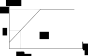
\includegraphics[width=\defaultwidth]{barral}
  \caption{Linear-saturated emission model from \citet{barral2003a}.}
  \label{fig-modelbarral}
\end{figure}

 We suppose that all of the electrons emitted are isotropically emitted following a Maxwellian flux distribution function of temperature $\Tsee$.
 The parameters $\proba_0$,  $\probamax$ and $\crover$ can be obtained from experiments. 
 \Cref{tab-seeparames} shows the crossover energy and the  probability of emission at energy null for different materials.
 The value of $\proba_0$ is always close to $0.5$, but $\crover$ can vary from 18 to 305 V.
 Hence, in the following parametric studies, $\proba_0$ will be kept at 0.5 while we vary $\crover$ from low values, corresponding to highly emmissive materials, to high values, representing less emmissive materials.
 
 \begin{table}[hbtp]
   \ra{1.3}
   \centering
   \caption{Emission parameters for different materials, from \citet{barral2003a}.}
   \label{tab-seeparames}
   \begin{tabular}{@{}lll@{}} \toprule
   Material & $\crover$ (V)& $\proba_0$ \\ \midrule
   BN-SiO$_2$ & 53 & 0.45 \\ 
   Al$_2$O$_3$ & 18  & 0.57 \\ 
   SiC     &  43  &0.69  \\
   Graphite & 305  & 0.40 \\ 
   \bottomrule
   \end{tabular}
 \end{table}
 
 Since the model used describe both the reflected and true secondary electron emission, we will use the general name \emph{electron emission}  to refer to the flux of electron comming from the wall toward the plasma.
 In contrast, the electrons reaching the plasma are referred to as the \emph{primary electrons}.

% !TEX root=/home/tavant/these/manuscript/src/manuscript.tex

\section{Study of electron cross field transport with a 2D radial-azimuthal PIC simulation}
  \label{sec-transport}
  
  \inlinenote{Rq de Anne: Mettre cette section sur la mobilite dans Chapter 0. Reponse: Ok, peut etre pas toutes les formules...? }
  \inlinenote{Anne: Revoir la transition, et mettre ici que les calcules numerique. L'état de l'art peut être ajouter au ch 0.}
  \inlinenote{Anne: transition ici à revoir....c'est un peu brutal : jusqu'ici on te suit car tu pars d'une description generale du PIC pour parler plus en detail des parois (Poisson, emission secondaire, gaine...)
Je pense que la premiere phrase de la 1.8 pourrait etre un truc du genre...
A key topic of my PhD work is to study the impact of surface processes on the plasma discharge and in particular on the electron mobility. }
  
  \inlinenote{Anne: je mettrai une grande partie du texte de cette page dans le chapitre 0 et je rappellerai ici juste les expressions de mu eff, mu classic, mu sat...et dire en 2 phrases comment ils sont calculés en PIC.}
  
  The electron mobility in the axial direction $\mobe$ is defined as the ratio between the mean velocity $u$ and the electric field
  \begin{equation} \label{eq-mudef}
    \mobe = \frac{u_{e,z}}{E_z}
  \end{equation}
  with $u_{e,z}=<v_{e,z}>$ the electron mean velocity.
  \nomenclature[Q]{\ensuremath{ u_{e,z}}}{Electron mean velocity in the axial direction\string: $u_{e,z} = < v_{e,z}>$}
  In the \ac{PIC} simulations, \cref{eq-mudef} can be used directly to compute $\mobpic$.
  
  In the classical drift diffusion theory of the electron mobility transverse to a magnetic field, the mobility is due to collisions as seen in \cref{eq-mobility} 
  \begin{equation} \label{eq-mobclas}
    \mobcla = \frac{e}{m_e} \frac{\nu_m}{\nu_m^2 + \oce^2}
  \end{equation}
  with $\oce=\frac{e B}{m_e}$ the electron cyclotron frequency and $\nu_m$ the electron-neutral momentum transfer collision frequency.
  \nomenclature[Q]{\ensuremath{ \oce}}{ Electron cyclotron frequency $\oce=\frac{e B}{m_e}$}
  \nomenclature[Q]{\ensuremath{ \nu_m}}{  electron-neutral momentum transfer collision frequency}
  
  At the exit plane, the classical mobility predicts a mobility of the order of $\mobcla=0.001-0.01\mobunit$ \citep{adam2008a}.
  
  The kinetic approach allowed \citet{lafleur2016a} to propose a modified mobility due to the oscillations of the electron density and the azimuthal electric field of the \ac{ECDI}.
  This effective mobility obtained is 
  \begin{equation} \label{eq-defmobeff}
    \mobeff = \mobcla \lp 1 - \frac{\oce}{\nu_m}  \frac{< \dne \dEt >_{\theta} }{n_0 E_z}   \rp
  \end{equation}
  with \dne{} and \dEt{} the fluctuations in the azimuthal directions of the electron density and azimuthal electric field, respectively, the operator $< . >_{\theta}$ is the average in the azimuthal direction, and $n_0$ is the average plasma density.
  In the case where $\nu_m << \oce$, \cref{eq-defmobeff} can be simplified to 
  \begin{align} 
    \mobeff &= \frac{\frac{e}{m_e} \nu_m}{\oce^2} \lp 1 - \frac{\oce^2}{\nu_m}  \frac{< \dne \dEt >_{\theta} }{n_0 E_z}   \rp \nonumber \\
    &= \frac{< \dne \dEt >_{\theta} }{n_0 E_z}   \frac{1}{B_r} \label{eq-mobeffsimple}
  \end{align}
  which shows that the instability enhances the electron axial mobility in a wave similar to an $E \times B$ drift.
  The electric field $E_{\theta}$ oscillates and presents a zero mean value, but the average effect on the electron transport is not zero if the correction between \dEt{} and \dne{} is not zero.
  
  In  \citet{lafleur2016a}, the authors present the instability effect as an electron-ion friction force $\Rei = - e < \dne \dEt >_{\theta}$.
  Under the assumption that the saturation of the instability is mainly due to ion trapping, the electron-ion friction force can be simplified in the \ac{2D} geometry of the simulation to
  \begin{equation} \label{eq-rei-sat}
    \Rei^{sat} = \frac{e \norm{\grad \cdot (n_e \Te \vect{v_i})}}{4 \sqrt{6} c_s} \simeq \frac{e n_e \Te \viout}{4 \sqrt 6 c_s L_z}
  \end{equation} 
  \nomenclature[Q]{\ensuremath{ \vect{v_i}}}{  ion velocity vector}
  \nomenclature[Q]{\ensuremath{ c_s}}{ ion sound speed $c_s=(e \Te/m_i)^{1/2}$ }
  where $\vect{v_i}$ is the ion velocity, $c_s=(e \Te/m_i)^{1/2}$  is the ion sound speed, and the spatial derivative in has been approximated across the axial simulation direction, with $\viout$ the ion outlet velocity 
  \begin{equation} \label{eq-viz}
    \viout = \sqrt{\frac{2 e U_z}{m_i}},
  \end{equation}
  with $U_z = E_z L_z$ the total potential difference in the axial direction.
  \nomenclature[Q]{\ensuremath{ U_z}}{   total potential difference in the axial direction $U_z = E_z L_z$}
  
  Using \cref{eq-rei-sat} in \cref{eq-mobeffsimple}, we obtain the simplified expression of the effective mobility at saturation
  \begin{equation} \label{eq-mobeffsat}
    \mobeffsat = \frac{\sqrt{\frac{\Te}{U_z}}}{4\sqrt{3}B_r}.
  \end{equation}
  
  \Cref{eq-mobeffsat} shows that for the radial and azimuthal \ac{2D} geometry being used here, the enhanced mobility due to \ac{ECDI} scales as the square-root of the electron temperature $\Te$ if the simulation parameters are constant.
  However, it is not the case in general, as the saturation of the instability can be also due to convection, and there are axial gradients in the electron temperature and plasma density as well.
  
  We can note that $\mobpic, \mobeff$ and $\mobcla$ are defined at every position of the simulation, but that $\mobeffsat$ can only be globally calculated. 
  
  
  
  
  
% !TEX root=/home/tavant/these/manuscript/src/manuscript.tex



\section{Conclusion}
  \label{sec-conclusion_ch1}
  
  In order to study the plasma wall interaction in an \ac{HET}, we developed a bi-dimensional simulation code using \ac{PIC}-\ac{MCC} modeling.
  As the electrons drift azimuthally due to the $E \times B$ configuration, the \ac{ECDI} rises, enhancing the cross field transport of the electron toward the anode.
  The walls closing the chamber in the radial direction are also important for the discharge behaviour.
  Hence, in order to compare the interaction between these phenomena, we simulate the radial-azimuthal domain.
  
  A special care have been taken concerning
  \begin{itemize}
    \item the modeling of the axial convection, in order to model the energy losses and so attain a steady state,
    \item the modeling of the radial boundary with the dielectric layer included in the simulation domain.
  \end{itemize}
  
  \inlinenote{Add a {\it typical result} to describe the may behaviour of the simulation ?}
  
  

% \acresetall
% !TEX root=/home/tavant/these/manuscript/src/manuscript.tex




\chapter{Parametric study of the dielectric characteristics}
\label{ch-2}
Structure :

{\bf II. Parametric study of the dielectric} 30 pages
\begin{zzz}
  This chapter takes the 1rst paper which uses Vivien's results.

  2.1 Fully metallic wall (no SEE, grounded).

  2.2 Impact of Dielectric layer without SEE

  2.3 Impact of SEE with grounded wall

  2.4 SEE and dielectric in the same time

  2.5 Discrepancy between $\mean{\Te}$, $\sigma_{PIC}$ and $\sigma_{theo} = \sigma_0 + (1 - \sigma_0) \frac{2 T_e}{\epsilon_0}$
\end{zzz}


In \Cref{ch-1}, we describe the simulation domain and the numerical models used.
As highlighted, the \ac{ECDI} rises due to the $E \times B$ electron drift, but saturate thanks to the axial convection model.
Before investigating the time dependent characteristics of the system, we focus in this \Cref{ch-2} on the average values at steady state.
A parametric study has been conducted on the radial boundary condition, on both the dielectric layer model in the Poisson equation, and the electron emission.


% !TEX root=/home/tavant/these/manuscript/src/manuscript.tex

\section{Canonical simulation results}
  \label{sec-canonical}
  
  The {\it canonical} case is the reference case that will be extensively described and commented.
  It will be used then to analyse and quantify the effects of the two aspect of the dielectric walls:
  \begin{itemize}
    \item the dielectric layer on the plasma potential, analysed in  % \cref{sec-dielectric_layer}
    \item the electron emission, analysed in %\cref{sec-see}
  \end{itemize}
  
  
  \Cref{fig-profiles} shows the radial profiles of the electron and ions densities averaged azimuthally.
  We can see the sheath close to the wall where the electron density fall rapidly compare to the ions.
  
  
  \begin{figure}[hbtp]
    \centering
    \includegraphics[width=\defaultwidth]{density_profile.pdf}
    \caption{Radial profile of the ion and electron densities at steady state.}
    \label{fig-profiles}
  \end{figure}
% !TEX root=/home/tavant/these/manuscript/src/manuscript.tex

\section{Conclusion}
  \label{sec-conclusion_ch2}
  

% \acresetall
% !TEX root=/home/tavant/these/manuscript/src/manuscript.tex




\chapter{Anisothermal sheath}
\label{ch-3}

In order to explain the discrepancy observed in \cref{ch-2} between the simulation and the sheath model, we investigate the simulation data.
We see that the hypothesis of the sheath model do not stand.
Using a simplified \ac{1D} \ac{PIC} simulation, we derive a polytropic closure for the electron.
With this new closure equation, we derived a modified sheath model, that fit well the kinetic simulations. 


{\bf III. Polytrotic sheath model} 23 pages
\begin{zzz}
  This chapter takes the 2nd paper about the modified sheath model

  3.1 EVDF in the 2D PIC simulations of HET.    3 pages

  3.2 1D simplified simulations, Parametric study and polytropic fits. 7 pages

  3.3 Monte-Carlo simulations.  3 pages

  3.4 fluid equations with polytropic closure. 10 pages
\end{zzz}


\minitoc




% !TEX root=/home/tavant/these/manuscript/src/manuscript.tex



\section{Insights for the PIC simulations}
\label{sec-insights}


% \acresetall
% !TEX root=/home/tavant/these/manuscript/src/manuscript.tex




\chapter{Polytropic sheath model in the presence of electron emission}
\label{ch-4}

\begin{Chabstract}
  
%e modify the polytropic sheath model with secondary electron emission
We add to the non-isothermal sheath model developed in \cref{ch-3} the secondary electron emission.
using the \ac{PIC} simulations, we observe that the polytropic index is almost constant when varying the cross-over energy $\crover$.
The predictions of the polytropic sheath model are compared to the \ac{PIC} simulations results presented in \cref{ch-2}.
The modified sheath model is included in a \ac{1D} fluid model.
\end{Chabstract}

{\bf IV. Polytrotic sheath model with SEE} 20 pages
\begin{zzz}
  This chapter goes beyond the actual modified sheath model in order to add SEEs.
  This require some time to develop before writting !

  5.1 Kinetic effects of the SEE on the EVDFs  4 pages

  5.2 SEE effects on the Fluid model  5 pages

  5.3 Validation against the Parametric 2D PIC simulation results. 2 pages
  
  5.4 1D fluid model with modified wall model. 4 pages
  
  5.4Bis Global model (Vivien's) with modified wall model. 4 pages
\end{zzz}

\minitoc
% 
% What is complicated here is the definition of the electron temperature, that include both primary and secondary electrons.
% Should we
% \begin{itemize}
%   \item Use a 2 fluid( so 1 electron) with a fluid model that includes the SEE ?
%   \item Use a 3 fluid model, that would  include folly absorbed primary electrons (simply polytropic) and emitted electrons, with strictly positive velocity.
% \end{itemize}
% 
% In the First case, the electron temperature is simple to define.
% But the closure equation may need to be changed.
% 
% the second case is more simpler, mathematicaly.
% 
% References:
% Il y a déjà eu beaucoup de travaux, mais aucun model fluides !
% 
% \citet{meezan2002} : Bolzmann solver, 2-Te EVDF, SEE compared with Maxwellian
% 
% \citet{smirnov2004} : MCC code, 2-Te EVDF. Mais fake EVDI effect via collisions
% 
% \citet{sydorenko2006a} : Beam in EVDF because of 1D PIC-MCC 
% 
% \citet{raitses2006} : "strong anisotropy : facteur 4",  compare Mesures avec fluids codes: says disagriment. Talks about 
% 
% \citet{ahedo2002} : sheath-presheath model with SEE with bolzmann electron, Sagdeev potential, SCL regime avec saturations 
% 
% \citet{ahedo2003} : 1D axial model avec wall interactions (SEE et SCL), plum with section increase (A(z)) 
% 
% \citet{ahedo2005} : Fluid model with SEE, with partial trapping and partial beams
% 
% \citet{raitses2005} : SCL regime and Te saturation (where he says that the SCL may not be responsible ??)
% 
% \citet{barral2003a} : 1D model, anisotrop electrons ({\bf must read to know how}), shows saturation at SCL with large anisotropy

{\bf \Large A lire}

\citet{sydorenko2007} :  non maxwellian EVDF

\citet{raitses2005a} : electron-wall interaction

\citet{jolivet2000} : SEE effect on EVDF 

% !TEX root=/home/tavant/these/manuscript/src/manuscript.tex


\section{Polytropic index in the \ac{HET} \ac{PIC} simulations}
\label{sec-PIC_poly}

\begin{figure}[hbtp]
  \centering
  \includegraphics[width=\defaultwidth]{EVDF_Bulk.pdf}
  \caption{Electron velocity distribution function at the center of the simulation, for different values of $\crover$.}
  \label{fig-evdf_epsstar}
\end{figure}

\begin{figure}[hbtp]
  \centering
  \includegraphics[width=\textwidth]{ne_Te_profiles.pdf}
  \caption{Radial profiles of (left) the electron density and (right) the electron temperature, for different values of $\crover$.}
  \label{fig-radial_profiles_see}
\end{figure}


\begin{figure}[hbtp]
  \centering
  \includegraphics[width=\defaultwidth]{SEE_polytropic_presheath_and_sheath.pdf}
  \caption{electron pressure as a function of the electron density normalized by the center variable, in log scale. Markers are every 10 cells (around 1$\lde$)}
  \label{fig-log_pe-ne}
\end{figure}

\renewcommand\subfigurewidth{3in}

\begin{figure}[hbtp]
  \centering
  \begin{tabular}{c c}
    \subfigure{SEE_polytropic_presheath}{a}{20,20} & 
    \subfigure{SEE_polyfit}{a}{20,20} 
  \end{tabular}
  \caption{Polytropic fit for different values of $\crover$. The sheath (10 cells) are removed from the plots.}
  \label{fig-polyfit_see}
\end{figure}

\FloatBarrier
{\bf Conclusion: $\gamma = 1.35$ in presheath and $\partial{\gamma} / \partial \crover = 0 $}

\paragraph{Hypothesis H1: } Polytropic model until the wall and $\gamma = 1.35$ (might be explained by \cref{{fig-evdf_epsstar}}, and by the fact that we care only on the forward temperature, so not distorted by the secondary electrons).

\paragraph{Hypothesis H2: } From {\bf H1}, and with the 2-$\Te$ hypothesis, we have $\rate = \rate_{\rm Maxw}(\Tew)$, were $\Tew$ can be computed from $Teb$, $\gamma$ and $\dphi$.

\paragraph{Hypothesis H3: } Current equality at the wall : $\Gamma_i + \rate \Gamma_e = \Gamma_e$. This is not a surprising hypothesis.

\section{Sheath model with polytropic electron and SEE}

With {\bf H1, H2} and {\bf H3} we have, as developed in \cref{sec-fluidPIC} with \cref{eq-gi,eq-ge,eq-tew}:
\begin{equation}\label{eq-sheathsee}
  (1 - \rate_{\rm Maxw}(\Tew) )\left[ 1 +\frac{\gamma -1}{\gamma} \frac{ \dphi_0}{ \Te_0}  \right]^{\frac{1}{\gamma - 1}} \sqrt{1 - \frac{\gamma -1}{\gamma}\frac{\dphi_0}{\Te_0}} = \sqrt{\frac{4 \gamma \pi m_e}{m_i}}
\end{equation}
In contrast with \cref{eq-sheath}, now the sheath potential $\Delta \phi$ depends on $\rate$ with depends on $\Te$.
Hence, $\dphi$ is not fully normalized.

\begin{figure}[hbtp]
  \centering
  \includegraphics[width=\defaultwidth]{Sheath_drop_with_SEE.pdf}
  \caption{Potential drop $\dphi$ normilized by the bulk electron temperature $\Te_0$ as a function of the polytropic index $\gamma$ for a xenon plasma ($m_i = 131\,\dalton$). The emission rate $\rate$ is fixed for clarity.}
  \label{fig-dphi_see}
\end{figure}

\begin{figure}[hbtp]
  \centering
  \includegraphics[width=\defaultwidth]{RSO_criteria_polytropic.pdf}
  \caption{ Plasma potential drop to the wall as a function of the electron temperature for different values of the cross-over energy $\crover$ using \cref{eq-sheathsee,eq-seemaxw}. The dashed line is $\dphi=\Te$. Similar to  \cref{fig-dphivsTe} but with polytropic electron of index $\gamma=1.35$}
  \label{fig-rso_crit_see}
\end{figure}

\FloatBarrier

\section{Comparison with PIC simulations} \label{subsec-picandmodel}

\begin{figure}[hbtp]
  \centering
  \includegraphics[width=\textwidth]{dphi_polytropic_noSEE}
  \caption{PIC simulation results (with SEE) compared to the polytropic limit without SEE.}
  \label{fig-polytropic_pic_noSEE}
\end{figure}

\begin{figure}[hbtp]
  \centering
  \includegraphics[width=\textwidth]{Summary_polytropic_SEE.pdf}
  \caption{Comparison of the PIC simulation results with the polytropic model with SEE.}
  \label{fig-polytropic_see_summary}
\end{figure}



% \acresetall
% !TEX root=/home/tavant/these/manuscript/src/manuscript.tex




\chapter{Anisothermal sheath}
\label{ch-3}

The presence of azimuthal instabilities in the Hall effect thrusters has first been showed with numerical simulations by \citet{adam2004}.
However, it nature is not yet fully understood.
In this chapter, we investigate the instabilities observed in the \ac{2D} \ac{PIC} simulations.

First, we derive the dispersion relation without hypothesis on the particle distribution function.
Then, we present a numerical algorithm that solves the dispersion relation using the distribution function measured in the \ac{PIC} simulations.
Then, the oscillations observed in the simulation are compared to the results of the dispersion relation.



{\bf V. analyse of the instability } 30 pages
\begin{zzz}
  \begin{itemize}
\item Instability dispersion relation
\item Kinetic solver for Ion and ECDI using VDFs
\item Impact of the difference w/r Maxwellian
\item Wall Boundary condition, 3D dispertion relation vs 1D and 2D relations
\item Linear stage as ECDI and Saturation toward IAW
\end{itemize}
\end{zzz}

\minitoc


\appendix


\backmatter
\let\leftmark=\oldleftmark
\let\rightmark=\oldrightmark
% \bibliographystyle{ieeetr}
% \newcommand*{\doi}[1]{\href{http://dx.doi.org/#1}{doi: \lstinline|#1|}}
% \newcommand*{\doi}[1]{\url{http://dx.doi.org/#1}}

\bibliographystyle{unsrtnatperso}  
% \bibliographystyle{theseen-nat-href}  
\bibliography{bib/MyLibrary}{}


% 
\pagestyle{empty}

%%% Logo de l'école doctorale. Le nom du fichier correspond au sigle de l'ED / Doctoral school logo. Filename correspond to doctoral school acronym
%%% Les noms valides sont / Valid names are : 2MIB; AAIF; ABIES; BIOSIGNE; CBMS; EDMH; EDOM; EDPIF; EDSP; EOBE; INTERFACES; ITFA; PHENIICS; SDSV; SDV; SHS; SMEMAG; SSMMH; STIC
\begin{textblock*}{61mm}(16mm,3mm)
	\noindent\includegraphics[height=24mm]{couvertures/ed/\logoEd.jpeg}
\end{textblock*}



%%%Titre de la thèse en français / Thesis title in french
\begin{center}
\fcolorbox{bordeau}{white}{\parbox{0.95\textwidth}{
{\bf Titre:} \PhDTitleFR
\medskip

%%%Mots clés en français, séprarés par des ; / Keywords in french, separated by ;
{\bf Mots clés:} \keywordsFR
\vspace{-2mm}

%%% Résumé en français / abstract in french
\begin{multicols}{2}
{\bf Résumé:}
\abstractFR
\end{multicols}
}}
\end{center}

\vspace*{0mm}

%%%Titre de la thèse en anglais / Thesis title in english
\begin{center}
\fcolorbox{bordeau}{white}{\parbox{0.95\textwidth}{
{\bf Title:} \PhDTitleEN

\medskip

%%%Mots clés en anglais, séprarés par des ; / Keywords in english, separated by ;
{\bf Keywords:}  \keywordsEN %%3 à 6 mots clés%%
\vspace{-2mm}
\begin{multicols}{2}

%%% Résumé en anglais / abstract in english
{\bf Abstract:}
\abstractEN
\end{multicols}
}}
\end{center}


\begin{textblock*}{161mm}(10mm,270mm)
\color{bordeau}
{\bf\noindent Université Paris-Saclay	         }

\noindent Espace Technologique / Immeuble Discovery

\noindent Route de l’Orme aux Merisiers RD 128 / 91190 Saint-Aubin, France
\end{textblock*}

\begin{textblock*}{20mm}(182mm,255mm)
\includegraphics[width=20mm]{couvertures/UPSACLAY-petit}
\end{textblock*}


\end{document}
